\documentclass[twoside]{book}

% Packages required by doxygen
\usepackage{fixltx2e}
\usepackage{calc}
\usepackage{doxygen}
\usepackage[export]{adjustbox} % also loads graphicx
\usepackage{graphicx}
\usepackage[utf8]{inputenc}
\usepackage{makeidx}
\usepackage{multicol}
\usepackage{multirow}
\PassOptionsToPackage{warn}{textcomp}
\usepackage{textcomp}
\usepackage[nointegrals]{wasysym}
\usepackage[table]{xcolor}

% Font selection
\usepackage[T1]{fontenc}
\usepackage[scaled=.90]{helvet}
\usepackage{courier}
\usepackage{amssymb}
\usepackage{sectsty}
\renewcommand{\familydefault}{\sfdefault}
\allsectionsfont{%
  \fontseries{bc}\selectfont%
  \color{darkgray}%
}
\renewcommand{\DoxyLabelFont}{%
  \fontseries{bc}\selectfont%
  \color{darkgray}%
}
\newcommand{\+}{\discretionary{\mbox{\scriptsize$\hookleftarrow$}}{}{}}

% Page & text layout
\usepackage{geometry}
\geometry{%
  a4paper,%
  top=2.5cm,%
  bottom=2.5cm,%
  left=2.5cm,%
  right=2.5cm%
}
\tolerance=750
\hfuzz=15pt
\hbadness=750
\setlength{\emergencystretch}{15pt}
\setlength{\parindent}{0cm}
\setlength{\parskip}{3ex plus 2ex minus 2ex}
\makeatletter
\renewcommand{\paragraph}{%
  \@startsection{paragraph}{4}{0ex}{-1.0ex}{1.0ex}{%
    \normalfont\normalsize\bfseries\SS@parafont%
  }%
}
\renewcommand{\subparagraph}{%
  \@startsection{subparagraph}{5}{0ex}{-1.0ex}{1.0ex}{%
    \normalfont\normalsize\bfseries\SS@subparafont%
  }%
}
\makeatother

% Headers & footers
\usepackage{fancyhdr}
\pagestyle{fancyplain}
\fancyhead[LE]{\fancyplain{}{\bfseries\thepage}}
\fancyhead[CE]{\fancyplain{}{}}
\fancyhead[RE]{\fancyplain{}{\bfseries\leftmark}}
\fancyhead[LO]{\fancyplain{}{\bfseries\rightmark}}
\fancyhead[CO]{\fancyplain{}{}}
\fancyhead[RO]{\fancyplain{}{\bfseries\thepage}}
\fancyfoot[LE]{\fancyplain{}{}}
\fancyfoot[CE]{\fancyplain{}{}}
\fancyfoot[RE]{\fancyplain{}{\bfseries\scriptsize Generated by Doxygen }}
\fancyfoot[LO]{\fancyplain{}{\bfseries\scriptsize Generated by Doxygen }}
\fancyfoot[CO]{\fancyplain{}{}}
\fancyfoot[RO]{\fancyplain{}{}}
\renewcommand{\footrulewidth}{0.4pt}
\renewcommand{\chaptermark}[1]{%
  \markboth{#1}{}%
}
\renewcommand{\sectionmark}[1]{%
  \markright{\thesection\ #1}%
}

% Indices & bibliography
\usepackage{natbib}
\usepackage[titles]{tocloft}
\setcounter{tocdepth}{3}
\setcounter{secnumdepth}{5}
\makeindex

% Hyperlinks (required, but should be loaded last)
\usepackage{ifpdf}
\ifpdf
  \usepackage[pdftex,pagebackref=true]{hyperref}
\else
  \usepackage[ps2pdf,pagebackref=true]{hyperref}
\fi
\hypersetup{%
  colorlinks=true,%
  linkcolor=blue,%
  citecolor=blue,%
  unicode%
}

% Custom commands
\newcommand{\clearemptydoublepage}{%
  \newpage{\pagestyle{empty}\cleardoublepage}%
}

\usepackage{caption}
\captionsetup{labelsep=space,justification=centering,font={bf},singlelinecheck=off,skip=4pt,position=top}

%===== C O N T E N T S =====

\begin{document}

% Titlepage & ToC
\hypersetup{pageanchor=false,
             bookmarksnumbered=true,
             pdfencoding=unicode
            }
\pagenumbering{alph}
\begin{titlepage}
\vspace*{7cm}
\begin{center}%
{\Large Isotope\+Fit\+Sharp \\[1ex]\large 1.\+0 }\\
\vspace*{1cm}
{\large Generated by Doxygen 1.8.13}\\
\end{center}
\end{titlepage}
\clearemptydoublepage
\pagenumbering{roman}
\tableofcontents
\clearemptydoublepage
\pagenumbering{arabic}
\hypersetup{pageanchor=true}

%--- Begin generated contents ---
\chapter{Namespace Index}
\section{Packages}
Here are the packages with brief descriptions (if available)\+:\begin{DoxyCompactList}
\item\contentsline{section}{\mbox{\hyperlink{namespace_isotope_fit}{Isotope\+Fit}} }{\pageref{namespace_isotope_fit}}{}
\end{DoxyCompactList}

\chapter{Hierarchical Index}
\section{Class Hierarchy}
This inheritance list is sorted roughly, but not completely, alphabetically\+:\begin{DoxyCompactList}
\item \contentsline{section}{Isotope\+Fit.\+I\+F\+Data.\+Baseline\+Corr}{\pageref{class_isotope_fit_1_1_i_f_data_1_1_baseline_corr}}{}
\item \contentsline{section}{Isotope\+Fit.\+I\+F\+Data.\+Calibration}{\pageref{class_isotope_fit_1_1_i_f_data_1_1_calibration}}{}
\item \contentsline{section}{Isotope\+Fit.\+I\+F\+Data.\+Cluster}{\pageref{class_isotope_fit_1_1_i_f_data_1_1_cluster}}{}
\item \contentsline{section}{Isotope\+Fit.\+Workspace.\+Design\+Mtrx}{\pageref{class_isotope_fit_1_1_workspace_1_1_design_mtrx}}{}
\item Exception\begin{DoxyCompactList}
\item \contentsline{section}{Isotope\+Fit.\+Interpolation.\+Interpolation\+Exception}{\pageref{class_isotope_fit_1_1_interpolation_1_1_interpolation_exception}}{}
\item \contentsline{section}{Isotope\+Fit.\+Workspace\+Exception}{\pageref{class_isotope_fit_1_1_workspace_exception}}{}
\end{DoxyCompactList}
\item \contentsline{section}{Isotope\+Fit.\+Interpolation}{\pageref{class_isotope_fit_1_1_interpolation}}{}
\begin{DoxyCompactList}
\item \contentsline{section}{Isotope\+Fit.\+Poly\+Interpolation}{\pageref{class_isotope_fit_1_1_poly_interpolation}}{}
\item \contentsline{section}{Isotope\+Fit.\+P\+P\+Interpolation}{\pageref{class_isotope_fit_1_1_p_p_interpolation}}{}
\end{DoxyCompactList}
\item \contentsline{section}{Isotope\+Fit.\+I\+F\+Data.\+Cluster.\+Isotope\+Data}{\pageref{class_isotope_fit_1_1_i_f_data_1_1_cluster_1_1_isotope_data}}{}
\item \contentsline{section}{Isotope\+Fit.\+Least\+Squares\+System}{\pageref{class_isotope_fit_1_1_least_squares_system}}{}
\item \contentsline{section}{Isotope\+Fit.\+I\+F\+Data.\+Calibration.\+Line\+Shape}{\pageref{class_isotope_fit_1_1_i_f_data_1_1_calibration_1_1_line_shape}}{}
\item \contentsline{section}{Isotope\+Fit.\+Pardiso}{\pageref{class_isotope_fit_1_1_pardiso}}{}
\item \contentsline{section}{Isotope\+Fit.\+I\+F\+Data.\+Spectrum}{\pageref{class_isotope_fit_1_1_i_f_data_1_1_spectrum}}{}
\item \contentsline{section}{Isotope\+Fit.\+S\+P\+QR}{\pageref{class_isotope_fit_1_1_s_p_q_r}}{}
\item \contentsline{section}{Isotope\+Fit.\+Workspace}{\pageref{class_isotope_fit_1_1_workspace}}{}
\item \contentsline{section}{Isotope\+Fit.\+Workspace.\+Workspace\+Status}{\pageref{class_isotope_fit_1_1_workspace_1_1_workspace_status}}{}
\end{DoxyCompactList}

\chapter{Class Index}
\section{Class List}
Here are the classes, structs, unions and interfaces with brief descriptions\+:\begin{DoxyCompactList}
\item\contentsline{section}{\hyperlink{class_isotope_fit_1_1_i_f_data_1_1_baseline_corr}{Isotope\+Fit.\+I\+F\+Data.\+Baseline\+Corr} \\*Class containing data for the baseline correction. }{\pageref{class_isotope_fit_1_1_i_f_data_1_1_baseline_corr}}{}
\item\contentsline{section}{\hyperlink{class_isotope_fit_1_1_i_f_data_1_1_calibration}{Isotope\+Fit.\+I\+F\+Data.\+Calibration} }{\pageref{class_isotope_fit_1_1_i_f_data_1_1_calibration}}{}
\item\contentsline{section}{\hyperlink{class_isotope_fit_1_1_i_f_data_1_1_cluster}{Isotope\+Fit.\+I\+F\+Data.\+Cluster} \\*Class for storing data about a single cluster/molecule/fragment. }{\pageref{class_isotope_fit_1_1_i_f_data_1_1_cluster}}{}
\item\contentsline{section}{\hyperlink{class_isotope_fit_1_1_workspace_1_1_design_mtrx}{Isotope\+Fit.\+Workspace.\+Design\+Mtrx} }{\pageref{class_isotope_fit_1_1_workspace_1_1_design_mtrx}}{}
\item\contentsline{section}{\hyperlink{class_isotope_fit_1_1_interpolation}{Isotope\+Fit.\+Interpolation} \\*Base class that handles data interpolations and related data. }{\pageref{class_isotope_fit_1_1_interpolation}}{}
\item\contentsline{section}{\hyperlink{class_isotope_fit_1_1_interpolation_1_1_interpolation_exception}{Isotope\+Fit.\+Interpolation.\+Interpolation\+Exception} }{\pageref{class_isotope_fit_1_1_interpolation_1_1_interpolation_exception}}{}
\item\contentsline{section}{\hyperlink{class_isotope_fit_1_1_i_f_data_1_1_cluster_1_1_isotope_data}{Isotope\+Fit.\+I\+F\+Data.\+Cluster.\+Isotope\+Data} \\*Class to store data about the isotopical pattern of a molecule/fragment. }{\pageref{class_isotope_fit_1_1_i_f_data_1_1_cluster_1_1_isotope_data}}{}
\item\contentsline{section}{\hyperlink{class_isotope_fit_1_1_least_squares_system}{Isotope\+Fit.\+Least\+Squares\+System} \\*Class for handling least squares systems. }{\pageref{class_isotope_fit_1_1_least_squares_system}}{}
\item\contentsline{section}{\hyperlink{class_isotope_fit_1_1_i_f_data_1_1_calibration_1_1_line_shape}{Isotope\+Fit.\+I\+F\+Data.\+Calibration.\+Line\+Shape} \\*Class containing the information about line shape. }{\pageref{class_isotope_fit_1_1_i_f_data_1_1_calibration_1_1_line_shape}}{}
\item\contentsline{section}{\hyperlink{class_isotope_fit_1_1_pardiso}{Isotope\+Fit.\+Pardiso} }{\pageref{class_isotope_fit_1_1_pardiso}}{}
\item\contentsline{section}{\hyperlink{class_isotope_fit_1_1_poly_interpolation}{Isotope\+Fit.\+Poly\+Interpolation} \\*Derived class that handles polynomial interpolations and evaluation of data. }{\pageref{class_isotope_fit_1_1_poly_interpolation}}{}
\item\contentsline{section}{\hyperlink{class_isotope_fit_1_1_p_p_interpolation}{Isotope\+Fit.\+P\+P\+Interpolation} \\*Derived class that handles piecewise polynomial interpolations and evaluation of data. }{\pageref{class_isotope_fit_1_1_p_p_interpolation}}{}
\item\contentsline{section}{\hyperlink{class_isotope_fit_1_1_i_f_data_1_1_spectrum}{Isotope\+Fit.\+I\+F\+Data.\+Spectrum} \\*Storage class for mass spectrum data. }{\pageref{class_isotope_fit_1_1_i_f_data_1_1_spectrum}}{}
\item\contentsline{section}{\hyperlink{class_isotope_fit_1_1_s_p_q_r}{Isotope\+Fit.\+S\+P\+QR} }{\pageref{class_isotope_fit_1_1_s_p_q_r}}{}
\item\contentsline{section}{\hyperlink{class_isotope_fit_1_1_workspace}{Isotope\+Fit.\+Workspace} \\*This class is the main interface for outside usage. }{\pageref{class_isotope_fit_1_1_workspace}}{}
\item\contentsline{section}{\hyperlink{class_isotope_fit_1_1_workspace_exception}{Isotope\+Fit.\+Workspace\+Exception} }{\pageref{class_isotope_fit_1_1_workspace_exception}}{}
\item\contentsline{section}{\hyperlink{class_isotope_fit_1_1_workspace_1_1_workspace_status}{Isotope\+Fit.\+Workspace.\+Workspace\+Status} \\*Class for storing the \hyperlink{class_isotope_fit_1_1_workspace}{Workspace} status flags and message log for the user. }{\pageref{class_isotope_fit_1_1_workspace_1_1_workspace_status}}{}
\end{DoxyCompactList}

\chapter{Namespace Documentation}
\hypertarget{namespace_isotope_fit}{}\section{Isotope\+Fit Namespace Reference}
\label{namespace_isotope_fit}\index{Isotope\+Fit@{Isotope\+Fit}}
\subsection*{Classes}
\begin{DoxyCompactItemize}
\item 
class {\bfseries Algorithm}
\item 
class {\bfseries I\+F\+Data}
\item 
class {\bfseries I\+F\+D\+File}
\item 
class \hyperlink{class_isotope_fit_1_1_interpolation}{Interpolation}
\begin{DoxyCompactList}\small\item\em Base class that handles data interpolations and related data. \end{DoxyCompactList}\item 
class \hyperlink{class_isotope_fit_1_1_least_squares_system}{Least\+Squares\+System}
\begin{DoxyCompactList}\small\item\em Class for handling least squares systems. \end{DoxyCompactList}\item 
class \hyperlink{class_isotope_fit_1_1_poly_interpolation}{Poly\+Interpolation}
\begin{DoxyCompactList}\small\item\em Derived class that handles polynomial interpolations and evaluation of data. \end{DoxyCompactList}\item 
class \hyperlink{class_isotope_fit_1_1_p_p_interpolation}{P\+P\+Interpolation}
\begin{DoxyCompactList}\small\item\em Derived class that handles piecewise polynomial interpolations and evaluation of data. \end{DoxyCompactList}\item 
class \hyperlink{class_isotope_fit_1_1_workspace}{Workspace}
\begin{DoxyCompactList}\small\item\em Hello \end{DoxyCompactList}\item 
class \hyperlink{class_isotope_fit_1_1_workspace_not_defined_exception}{Workspace\+Not\+Defined\+Exception}
\end{DoxyCompactItemize}

\chapter{Class Documentation}
\hypertarget{class_isotope_fit_1_1_i_f_data_1_1_baseline_corr}{}\section{Isotope\+Fit.\+I\+F\+Data.\+Baseline\+Corr Class Reference}
\label{class_isotope_fit_1_1_i_f_data_1_1_baseline_corr}\index{Isotope\+Fit.\+I\+F\+Data.\+Baseline\+Corr@{Isotope\+Fit.\+I\+F\+Data.\+Baseline\+Corr}}


Class containing data for the baseline correction.  


\subsection*{Properties}
\begin{DoxyCompactItemize}
\item 
\mbox{\Hypertarget{class_isotope_fit_1_1_i_f_data_1_1_baseline_corr_a90e35ea8c62d07f0279f4b5f7d440491}\label{class_isotope_fit_1_1_i_f_data_1_1_baseline_corr_a90e35ea8c62d07f0279f4b5f7d440491}} 
double \mbox{[}$\,$\mbox{]} \hyperlink{class_isotope_fit_1_1_i_f_data_1_1_baseline_corr_a90e35ea8c62d07f0279f4b5f7d440491}{X\+Axis}\hspace{0.3cm}{\ttfamily  \mbox{[}get, set\mbox{]}}
\begin{DoxyCompactList}\small\item\em X-\/values of the baseline correction points. \end{DoxyCompactList}\item 
double \mbox{[}$\,$\mbox{]} \hyperlink{class_isotope_fit_1_1_i_f_data_1_1_baseline_corr_aa71067f79827da27836daa705413133c}{Y\+Axis}\hspace{0.3cm}{\ttfamily  \mbox{[}get, set\mbox{]}}
\begin{DoxyCompactList}\small\item\em Y-\/values of the baseline correction points. \end{DoxyCompactList}\item 
\hyperlink{class_isotope_fit_1_1_interpolation}{Interpolation} \hyperlink{class_isotope_fit_1_1_i_f_data_1_1_baseline_corr_a914a7b2ac945482a7c73874fbff45951}{Baseline\+Interpolation}\hspace{0.3cm}{\ttfamily  \mbox{[}get, set\mbox{]}}
\begin{DoxyCompactList}\small\item\em Object containing results of the baseline interpolation. \end{DoxyCompactList}\end{DoxyCompactItemize}


\subsection{Detailed Description}
Class containing data for the baseline correction. 



Definition at line 338 of file I\+F\+Data.\+cs.



\subsection{Property Documentation}
\mbox{\Hypertarget{class_isotope_fit_1_1_i_f_data_1_1_baseline_corr_a914a7b2ac945482a7c73874fbff45951}\label{class_isotope_fit_1_1_i_f_data_1_1_baseline_corr_a914a7b2ac945482a7c73874fbff45951}} 
\index{Isotope\+Fit\+::\+I\+F\+Data\+::\+Baseline\+Corr@{Isotope\+Fit\+::\+I\+F\+Data\+::\+Baseline\+Corr}!Baseline\+Interpolation@{Baseline\+Interpolation}}
\index{Baseline\+Interpolation@{Baseline\+Interpolation}!Isotope\+Fit\+::\+I\+F\+Data\+::\+Baseline\+Corr@{Isotope\+Fit\+::\+I\+F\+Data\+::\+Baseline\+Corr}}
\subsubsection{\texorpdfstring{Baseline\+Interpolation}{BaselineInterpolation}}
{\footnotesize\ttfamily \hyperlink{class_isotope_fit_1_1_interpolation}{Interpolation} Isotope\+Fit.\+I\+F\+Data.\+Baseline\+Corr.\+Baseline\+Interpolation\hspace{0.3cm}{\ttfamily [get]}, {\ttfamily [set]}}



Object containing results of the baseline interpolation. 



Definition at line 357 of file I\+F\+Data.\+cs.

\mbox{\Hypertarget{class_isotope_fit_1_1_i_f_data_1_1_baseline_corr_aa71067f79827da27836daa705413133c}\label{class_isotope_fit_1_1_i_f_data_1_1_baseline_corr_aa71067f79827da27836daa705413133c}} 
\index{Isotope\+Fit\+::\+I\+F\+Data\+::\+Baseline\+Corr@{Isotope\+Fit\+::\+I\+F\+Data\+::\+Baseline\+Corr}!Y\+Axis@{Y\+Axis}}
\index{Y\+Axis@{Y\+Axis}!Isotope\+Fit\+::\+I\+F\+Data\+::\+Baseline\+Corr@{Isotope\+Fit\+::\+I\+F\+Data\+::\+Baseline\+Corr}}
\subsubsection{\texorpdfstring{Y\+Axis}{YAxis}}
{\footnotesize\ttfamily double \mbox{[}$\,$\mbox{]} Isotope\+Fit.\+I\+F\+Data.\+Baseline\+Corr.\+Y\+Axis\hspace{0.3cm}{\ttfamily [get]}, {\ttfamily [set]}}



Y-\/values of the baseline correction points. 



Definition at line 352 of file I\+F\+Data.\+cs.



The documentation for this class was generated from the following file\+:\begin{DoxyCompactItemize}
\item 
Isotope\+Fit\+Lib/I\+F\+Data.\+cs\end{DoxyCompactItemize}

\hypertarget{class_isotope_fit_1_1_i_f_data_1_1_calibration}{}\section{Isotope\+Fit.\+I\+F\+Data.\+Calibration Class Reference}
\label{class_isotope_fit_1_1_i_f_data_1_1_calibration}\index{Isotope\+Fit.\+I\+F\+Data.\+Calibration@{Isotope\+Fit.\+I\+F\+Data.\+Calibration}}
\subsection*{Classes}
\begin{DoxyCompactItemize}
\item 
class \mbox{\hyperlink{class_isotope_fit_1_1_i_f_data_1_1_calibration_1_1_line_shape}{Line\+Shape}}
\begin{DoxyCompactList}\small\item\em Class containing the information about line shape. \end{DoxyCompactList}\end{DoxyCompactItemize}
\subsection*{Properties}
\begin{DoxyCompactItemize}
\item 
\mbox{\Hypertarget{class_isotope_fit_1_1_i_f_data_1_1_calibration_ae73e31f6527fdfc9cb05851283c91abf}\label{class_isotope_fit_1_1_i_f_data_1_1_calibration_ae73e31f6527fdfc9cb05851283c91abf}} 
double \mbox{[}$\,$\mbox{]} {\bfseries C\+O\+M\+List}\hspace{0.3cm}{\ttfamily  \mbox{[}get, set\mbox{]}}
\item 
\mbox{\Hypertarget{class_isotope_fit_1_1_i_f_data_1_1_calibration_a66fbb2c3d26c1da7de8dd797f62bdcff}\label{class_isotope_fit_1_1_i_f_data_1_1_calibration_a66fbb2c3d26c1da7de8dd797f62bdcff}} 
double \mbox{[}$\,$\mbox{]} {\bfseries Mass\+Offset\+List}\hspace{0.3cm}{\ttfamily  \mbox{[}get, set\mbox{]}}
\item 
\mbox{\Hypertarget{class_isotope_fit_1_1_i_f_data_1_1_calibration_ae4a019657f9c856274b577aee30ed140}\label{class_isotope_fit_1_1_i_f_data_1_1_calibration_ae4a019657f9c856274b577aee30ed140}} 
double \mbox{[}$\,$\mbox{]} {\bfseries Resolution\+List}\hspace{0.3cm}{\ttfamily  \mbox{[}get, set\mbox{]}}
\item 
\mbox{\Hypertarget{class_isotope_fit_1_1_i_f_data_1_1_calibration_a3fd5fabda47ec06b75abe741a959a640}\label{class_isotope_fit_1_1_i_f_data_1_1_calibration_a3fd5fabda47ec06b75abe741a959a640}} 
string {\bfseries Mass\+Offset\+Method}\hspace{0.3cm}{\ttfamily  \mbox{[}get, set\mbox{]}}
\item 
\mbox{\Hypertarget{class_isotope_fit_1_1_i_f_data_1_1_calibration_a1d0576963ddb1bd5dee63fe05ee2ba88}\label{class_isotope_fit_1_1_i_f_data_1_1_calibration_a1d0576963ddb1bd5dee63fe05ee2ba88}} 
string {\bfseries Resolution\+Method}\hspace{0.3cm}{\ttfamily  \mbox{[}get, set\mbox{]}}
\item 
\mbox{\Hypertarget{class_isotope_fit_1_1_i_f_data_1_1_calibration_a43c6a104771e41ef627ffbeefc745ad3}\label{class_isotope_fit_1_1_i_f_data_1_1_calibration_a43c6a104771e41ef627ffbeefc745ad3}} 
int {\bfseries Mass\+Offset\+Param}\hspace{0.3cm}{\ttfamily  \mbox{[}get, set\mbox{]}}
\item 
\mbox{\Hypertarget{class_isotope_fit_1_1_i_f_data_1_1_calibration_ac215515a411ade3f25b2828589ca32d7}\label{class_isotope_fit_1_1_i_f_data_1_1_calibration_ac215515a411ade3f25b2828589ca32d7}} 
int {\bfseries Resolution\+Param}\hspace{0.3cm}{\ttfamily  \mbox{[}get, set\mbox{]}}
\item 
List$<$ string $>$ \mbox{\hyperlink{class_isotope_fit_1_1_i_f_data_1_1_calibration_a2e347f087df878f22010302bda7db4be}{Name\+List}}\hspace{0.3cm}{\ttfamily  \mbox{[}get, set\mbox{]}}
\begin{DoxyCompactList}\small\item\em List of I\+Ds of clusters picked as calibration points for mass offset and resolution. \end{DoxyCompactList}\item 
\mbox{\hyperlink{class_isotope_fit_1_1_i_f_data_1_1_calibration_1_1_line_shape}{Line\+Shape}} \mbox{\hyperlink{class_isotope_fit_1_1_i_f_data_1_1_calibration_ad0c3e0969448ad0cc57307c77c2222eb}{Shape}}\hspace{0.3cm}{\ttfamily  \mbox{[}get, set\mbox{]}}
\begin{DoxyCompactList}\small\item\em Object containing the information about the line shape. \end{DoxyCompactList}\item 
\mbox{\hyperlink{class_isotope_fit_1_1_interpolation}{Interpolation}} \mbox{\hyperlink{class_isotope_fit_1_1_i_f_data_1_1_calibration_af383c1c97a369e786e72ac5d79e8973e}{Mass\+Offset\+Interp}}\hspace{0.3cm}{\ttfamily  \mbox{[}get, set\mbox{]}}
\begin{DoxyCompactList}\small\item\em Object containing the results of mass offset interpolation. \end{DoxyCompactList}\item 
\mbox{\hyperlink{class_isotope_fit_1_1_interpolation}{Interpolation}} \mbox{\hyperlink{class_isotope_fit_1_1_i_f_data_1_1_calibration_ab8db2fa10ee3de8f8deca251f4bd3518}{Resolution\+Interp}}\hspace{0.3cm}{\ttfamily  \mbox{[}get, set\mbox{]}}
\begin{DoxyCompactList}\small\item\em Object containing the results of resolution fit. \end{DoxyCompactList}\end{DoxyCompactItemize}


\subsection{Detailed Description}


Definition at line 305 of file I\+F\+Data.\+cs.



\subsection{Property Documentation}
\mbox{\Hypertarget{class_isotope_fit_1_1_i_f_data_1_1_calibration_af383c1c97a369e786e72ac5d79e8973e}\label{class_isotope_fit_1_1_i_f_data_1_1_calibration_af383c1c97a369e786e72ac5d79e8973e}} 
\index{Isotope\+Fit\+::\+I\+F\+Data\+::\+Calibration@{Isotope\+Fit\+::\+I\+F\+Data\+::\+Calibration}!Mass\+Offset\+Interp@{Mass\+Offset\+Interp}}
\index{Mass\+Offset\+Interp@{Mass\+Offset\+Interp}!Isotope\+Fit\+::\+I\+F\+Data\+::\+Calibration@{Isotope\+Fit\+::\+I\+F\+Data\+::\+Calibration}}
\subsubsection{\texorpdfstring{Mass\+Offset\+Interp}{MassOffsetInterp}}
{\footnotesize\ttfamily \mbox{\hyperlink{class_isotope_fit_1_1_interpolation}{Interpolation}} Isotope\+Fit.\+I\+F\+Data.\+Calibration.\+Mass\+Offset\+Interp\hspace{0.3cm}{\ttfamily [get]}, {\ttfamily [set]}}



Object containing the results of mass offset interpolation. 



Definition at line 328 of file I\+F\+Data.\+cs.

\mbox{\Hypertarget{class_isotope_fit_1_1_i_f_data_1_1_calibration_a2e347f087df878f22010302bda7db4be}\label{class_isotope_fit_1_1_i_f_data_1_1_calibration_a2e347f087df878f22010302bda7db4be}} 
\index{Isotope\+Fit\+::\+I\+F\+Data\+::\+Calibration@{Isotope\+Fit\+::\+I\+F\+Data\+::\+Calibration}!Name\+List@{Name\+List}}
\index{Name\+List@{Name\+List}!Isotope\+Fit\+::\+I\+F\+Data\+::\+Calibration@{Isotope\+Fit\+::\+I\+F\+Data\+::\+Calibration}}
\subsubsection{\texorpdfstring{Name\+List}{NameList}}
{\footnotesize\ttfamily List$<$string$>$ Isotope\+Fit.\+I\+F\+Data.\+Calibration.\+Name\+List\hspace{0.3cm}{\ttfamily [get]}, {\ttfamily [set]}}



List of I\+Ds of clusters picked as calibration points for mass offset and resolution. 



Definition at line 318 of file I\+F\+Data.\+cs.

\mbox{\Hypertarget{class_isotope_fit_1_1_i_f_data_1_1_calibration_ab8db2fa10ee3de8f8deca251f4bd3518}\label{class_isotope_fit_1_1_i_f_data_1_1_calibration_ab8db2fa10ee3de8f8deca251f4bd3518}} 
\index{Isotope\+Fit\+::\+I\+F\+Data\+::\+Calibration@{Isotope\+Fit\+::\+I\+F\+Data\+::\+Calibration}!Resolution\+Interp@{Resolution\+Interp}}
\index{Resolution\+Interp@{Resolution\+Interp}!Isotope\+Fit\+::\+I\+F\+Data\+::\+Calibration@{Isotope\+Fit\+::\+I\+F\+Data\+::\+Calibration}}
\subsubsection{\texorpdfstring{Resolution\+Interp}{ResolutionInterp}}
{\footnotesize\ttfamily \mbox{\hyperlink{class_isotope_fit_1_1_interpolation}{Interpolation}} Isotope\+Fit.\+I\+F\+Data.\+Calibration.\+Resolution\+Interp\hspace{0.3cm}{\ttfamily [get]}, {\ttfamily [set]}}



Object containing the results of resolution fit. 



Definition at line 333 of file I\+F\+Data.\+cs.

\mbox{\Hypertarget{class_isotope_fit_1_1_i_f_data_1_1_calibration_ad0c3e0969448ad0cc57307c77c2222eb}\label{class_isotope_fit_1_1_i_f_data_1_1_calibration_ad0c3e0969448ad0cc57307c77c2222eb}} 
\index{Isotope\+Fit\+::\+I\+F\+Data\+::\+Calibration@{Isotope\+Fit\+::\+I\+F\+Data\+::\+Calibration}!Shape@{Shape}}
\index{Shape@{Shape}!Isotope\+Fit\+::\+I\+F\+Data\+::\+Calibration@{Isotope\+Fit\+::\+I\+F\+Data\+::\+Calibration}}
\subsubsection{\texorpdfstring{Shape}{Shape}}
{\footnotesize\ttfamily \mbox{\hyperlink{class_isotope_fit_1_1_i_f_data_1_1_calibration_1_1_line_shape}{Line\+Shape}} Isotope\+Fit.\+I\+F\+Data.\+Calibration.\+Shape\hspace{0.3cm}{\ttfamily [get]}, {\ttfamily [set]}}



Object containing the information about the line shape. 



Definition at line 323 of file I\+F\+Data.\+cs.



The documentation for this class was generated from the following file\+:\begin{DoxyCompactItemize}
\item 
Isotope\+Fit\+Lib/I\+F\+Data.\+cs\end{DoxyCompactItemize}

\hypertarget{class_isotope_fit_1_1_i_f_data_1_1_cluster}{}\section{Isotope\+Fit.\+I\+F\+Data.\+Cluster Class Reference}
\label{class_isotope_fit_1_1_i_f_data_1_1_cluster}\index{Isotope\+Fit.\+I\+F\+Data.\+Cluster@{Isotope\+Fit.\+I\+F\+Data.\+Cluster}}


Class for storing data about a single cluster/molecule/fragment.  


\subsection*{Classes}
\begin{DoxyCompactItemize}
\item 
class \mbox{\hyperlink{class_isotope_fit_1_1_i_f_data_1_1_cluster_1_1_isotope_data}{Isotope\+Data}}
\begin{DoxyCompactList}\small\item\em Class to store data about the isotopical pattern of a molecule/fragment. \end{DoxyCompactList}\end{DoxyCompactItemize}
\subsection*{Public Member Functions}
\begin{DoxyCompactItemize}
\item 
\mbox{\hyperlink{class_isotope_fit_1_1_i_f_data_1_1_cluster_ada019f0710b46fddad5f74a541deb4da}{Cluster}} ()
\begin{DoxyCompactList}\small\item\em Creates an empty cluster object. \end{DoxyCompactList}\end{DoxyCompactItemize}
\subsection*{Properties}
\begin{DoxyCompactItemize}
\item 
\mbox{\hyperlink{class_isotope_fit_1_1_i_f_data_1_1_cluster_1_1_isotope_data}{Isotope\+Data}} \mbox{\hyperlink{class_isotope_fit_1_1_i_f_data_1_1_cluster_a9874ca075e89c301587ef9cdc1d7a5c6}{Peak\+Data}}\hspace{0.3cm}{\ttfamily  \mbox{[}get, set\mbox{]}}
\begin{DoxyCompactList}\small\item\em Stores the isotopical data for the cluster. \end{DoxyCompactList}\item 
string \mbox{\hyperlink{class_isotope_fit_1_1_i_f_data_1_1_cluster_a8ae80358415b5637dbe46d2a211d03e7}{Name}}\hspace{0.3cm}{\ttfamily  \mbox{[}get, set\mbox{]}}
\begin{DoxyCompactList}\small\item\em Human readable name of the cluster. N\+OT the I\+D! \end{DoxyCompactList}\item 
double \mbox{\hyperlink{class_isotope_fit_1_1_i_f_data_1_1_cluster_a43d9e77aebe1e02b617b16aff448c613}{Centre\+Of\+Mass}}\hspace{0.3cm}{\ttfamily  \mbox{[}get, set\mbox{]}}
\begin{DoxyCompactList}\small\item\em Centre of mass of the cluster, used for mass offset correction. \end{DoxyCompactList}\item 
double \mbox{\hyperlink{class_isotope_fit_1_1_i_f_data_1_1_cluster_ac7dbcceda366fd00ce0c12f1cdd35fea}{Abundance}}\hspace{0.3cm}{\ttfamily  \mbox{[}get, set\mbox{]}}
\begin{DoxyCompactList}\small\item\em Fitted abundance of the cluster. \end{DoxyCompactList}\item 
double \mbox{\hyperlink{class_isotope_fit_1_1_i_f_data_1_1_cluster_a3658f5cbf7c18d18af2164998c30661f}{Abundance\+Error}}\hspace{0.3cm}{\ttfamily  \mbox{[}get, set\mbox{]}}
\begin{DoxyCompactList}\small\item\em Error of the fitted abundance value. \end{DoxyCompactList}\item 
double \mbox{\hyperlink{class_isotope_fit_1_1_i_f_data_1_1_cluster_afa64046ba8bdad51edc7ca5c1c39cd8c}{Mass\+Offset}}\hspace{0.3cm}{\ttfamily  \mbox{[}get, set\mbox{]}}
\begin{DoxyCompactList}\small\item\em Mass offset of the cluster, used for mass offset correction. \end{DoxyCompactList}\item 
double \mbox{\hyperlink{class_isotope_fit_1_1_i_f_data_1_1_cluster_ad98e129dd08bfd98df4b474b4c9139f8}{Resolution}}\hspace{0.3cm}{\ttfamily  \mbox{[}get, set\mbox{]}}
\begin{DoxyCompactList}\small\item\em Resolution of the particular cluster line, used for resolution calibration. \end{DoxyCompactList}\end{DoxyCompactItemize}


\subsection{Detailed Description}
Class for storing data about a single cluster/molecule/fragment. 



Definition at line 186 of file I\+F\+Data.\+cs.



\subsection{Constructor \& Destructor Documentation}
\mbox{\Hypertarget{class_isotope_fit_1_1_i_f_data_1_1_cluster_ada019f0710b46fddad5f74a541deb4da}\label{class_isotope_fit_1_1_i_f_data_1_1_cluster_ada019f0710b46fddad5f74a541deb4da}} 
\index{Isotope\+Fit\+::\+I\+F\+Data\+::\+Cluster@{Isotope\+Fit\+::\+I\+F\+Data\+::\+Cluster}!Cluster@{Cluster}}
\index{Cluster@{Cluster}!Isotope\+Fit\+::\+I\+F\+Data\+::\+Cluster@{Isotope\+Fit\+::\+I\+F\+Data\+::\+Cluster}}
\subsubsection{\texorpdfstring{Cluster()}{Cluster()}}
{\footnotesize\ttfamily Isotope\+Fit.\+I\+F\+Data.\+Cluster.\+Cluster (\begin{DoxyParamCaption}{ }\end{DoxyParamCaption})}



Creates an empty cluster object. 



Definition at line 245 of file I\+F\+Data.\+cs.



\subsection{Property Documentation}
\mbox{\Hypertarget{class_isotope_fit_1_1_i_f_data_1_1_cluster_ac7dbcceda366fd00ce0c12f1cdd35fea}\label{class_isotope_fit_1_1_i_f_data_1_1_cluster_ac7dbcceda366fd00ce0c12f1cdd35fea}} 
\index{Isotope\+Fit\+::\+I\+F\+Data\+::\+Cluster@{Isotope\+Fit\+::\+I\+F\+Data\+::\+Cluster}!Abundance@{Abundance}}
\index{Abundance@{Abundance}!Isotope\+Fit\+::\+I\+F\+Data\+::\+Cluster@{Isotope\+Fit\+::\+I\+F\+Data\+::\+Cluster}}
\subsubsection{\texorpdfstring{Abundance}{Abundance}}
{\footnotesize\ttfamily double Isotope\+Fit.\+I\+F\+Data.\+Cluster.\+Abundance\hspace{0.3cm}{\ttfamily [get]}, {\ttfamily [set]}}



Fitted abundance of the cluster. 



Definition at line 216 of file I\+F\+Data.\+cs.

\mbox{\Hypertarget{class_isotope_fit_1_1_i_f_data_1_1_cluster_a3658f5cbf7c18d18af2164998c30661f}\label{class_isotope_fit_1_1_i_f_data_1_1_cluster_a3658f5cbf7c18d18af2164998c30661f}} 
\index{Isotope\+Fit\+::\+I\+F\+Data\+::\+Cluster@{Isotope\+Fit\+::\+I\+F\+Data\+::\+Cluster}!Abundance\+Error@{Abundance\+Error}}
\index{Abundance\+Error@{Abundance\+Error}!Isotope\+Fit\+::\+I\+F\+Data\+::\+Cluster@{Isotope\+Fit\+::\+I\+F\+Data\+::\+Cluster}}
\subsubsection{\texorpdfstring{Abundance\+Error}{AbundanceError}}
{\footnotesize\ttfamily double Isotope\+Fit.\+I\+F\+Data.\+Cluster.\+Abundance\+Error\hspace{0.3cm}{\ttfamily [get]}, {\ttfamily [set]}}



Error of the fitted abundance value. 



Definition at line 221 of file I\+F\+Data.\+cs.

\mbox{\Hypertarget{class_isotope_fit_1_1_i_f_data_1_1_cluster_a43d9e77aebe1e02b617b16aff448c613}\label{class_isotope_fit_1_1_i_f_data_1_1_cluster_a43d9e77aebe1e02b617b16aff448c613}} 
\index{Isotope\+Fit\+::\+I\+F\+Data\+::\+Cluster@{Isotope\+Fit\+::\+I\+F\+Data\+::\+Cluster}!Centre\+Of\+Mass@{Centre\+Of\+Mass}}
\index{Centre\+Of\+Mass@{Centre\+Of\+Mass}!Isotope\+Fit\+::\+I\+F\+Data\+::\+Cluster@{Isotope\+Fit\+::\+I\+F\+Data\+::\+Cluster}}
\subsubsection{\texorpdfstring{Centre\+Of\+Mass}{CentreOfMass}}
{\footnotesize\ttfamily double Isotope\+Fit.\+I\+F\+Data.\+Cluster.\+Centre\+Of\+Mass\hspace{0.3cm}{\ttfamily [get]}, {\ttfamily [set]}}



Centre of mass of the cluster, used for mass offset correction. 

This value needs to be set only for those clusters, that were chosen as calibration clusters by the \mbox{\hyperlink{class_isotope_fit_1_1_i_f_data_1_1_calibration_a2e347f087df878f22010302bda7db4be}{Calibration.\+Name\+List}} ID list. 

Definition at line 207 of file I\+F\+Data.\+cs.

\mbox{\Hypertarget{class_isotope_fit_1_1_i_f_data_1_1_cluster_afa64046ba8bdad51edc7ca5c1c39cd8c}\label{class_isotope_fit_1_1_i_f_data_1_1_cluster_afa64046ba8bdad51edc7ca5c1c39cd8c}} 
\index{Isotope\+Fit\+::\+I\+F\+Data\+::\+Cluster@{Isotope\+Fit\+::\+I\+F\+Data\+::\+Cluster}!Mass\+Offset@{Mass\+Offset}}
\index{Mass\+Offset@{Mass\+Offset}!Isotope\+Fit\+::\+I\+F\+Data\+::\+Cluster@{Isotope\+Fit\+::\+I\+F\+Data\+::\+Cluster}}
\subsubsection{\texorpdfstring{Mass\+Offset}{MassOffset}}
{\footnotesize\ttfamily double Isotope\+Fit.\+I\+F\+Data.\+Cluster.\+Mass\+Offset\hspace{0.3cm}{\ttfamily [get]}, {\ttfamily [set]}}



Mass offset of the cluster, used for mass offset correction. 

This value needs to be set only for those clusters, that were chosen as calibration clusters by the \mbox{\hyperlink{class_isotope_fit_1_1_i_f_data_1_1_calibration_a2e347f087df878f22010302bda7db4be}{Calibration.\+Name\+List}} ID list. 

Definition at line 229 of file I\+F\+Data.\+cs.

\mbox{\Hypertarget{class_isotope_fit_1_1_i_f_data_1_1_cluster_a8ae80358415b5637dbe46d2a211d03e7}\label{class_isotope_fit_1_1_i_f_data_1_1_cluster_a8ae80358415b5637dbe46d2a211d03e7}} 
\index{Isotope\+Fit\+::\+I\+F\+Data\+::\+Cluster@{Isotope\+Fit\+::\+I\+F\+Data\+::\+Cluster}!Name@{Name}}
\index{Name@{Name}!Isotope\+Fit\+::\+I\+F\+Data\+::\+Cluster@{Isotope\+Fit\+::\+I\+F\+Data\+::\+Cluster}}
\subsubsection{\texorpdfstring{Name}{Name}}
{\footnotesize\ttfamily string Isotope\+Fit.\+I\+F\+Data.\+Cluster.\+Name\hspace{0.3cm}{\ttfamily [get]}, {\ttfamily [set]}}



Human readable name of the cluster. N\+OT the I\+D! 



Definition at line 196 of file I\+F\+Data.\+cs.

\mbox{\Hypertarget{class_isotope_fit_1_1_i_f_data_1_1_cluster_a9874ca075e89c301587ef9cdc1d7a5c6}\label{class_isotope_fit_1_1_i_f_data_1_1_cluster_a9874ca075e89c301587ef9cdc1d7a5c6}} 
\index{Isotope\+Fit\+::\+I\+F\+Data\+::\+Cluster@{Isotope\+Fit\+::\+I\+F\+Data\+::\+Cluster}!Peak\+Data@{Peak\+Data}}
\index{Peak\+Data@{Peak\+Data}!Isotope\+Fit\+::\+I\+F\+Data\+::\+Cluster@{Isotope\+Fit\+::\+I\+F\+Data\+::\+Cluster}}
\subsubsection{\texorpdfstring{Peak\+Data}{PeakData}}
{\footnotesize\ttfamily \mbox{\hyperlink{class_isotope_fit_1_1_i_f_data_1_1_cluster_1_1_isotope_data}{Isotope\+Data}} Isotope\+Fit.\+I\+F\+Data.\+Cluster.\+Peak\+Data\hspace{0.3cm}{\ttfamily [get]}, {\ttfamily [set]}}



Stores the isotopical data for the cluster. 



Definition at line 191 of file I\+F\+Data.\+cs.

\mbox{\Hypertarget{class_isotope_fit_1_1_i_f_data_1_1_cluster_ad98e129dd08bfd98df4b474b4c9139f8}\label{class_isotope_fit_1_1_i_f_data_1_1_cluster_ad98e129dd08bfd98df4b474b4c9139f8}} 
\index{Isotope\+Fit\+::\+I\+F\+Data\+::\+Cluster@{Isotope\+Fit\+::\+I\+F\+Data\+::\+Cluster}!Resolution@{Resolution}}
\index{Resolution@{Resolution}!Isotope\+Fit\+::\+I\+F\+Data\+::\+Cluster@{Isotope\+Fit\+::\+I\+F\+Data\+::\+Cluster}}
\subsubsection{\texorpdfstring{Resolution}{Resolution}}
{\footnotesize\ttfamily double Isotope\+Fit.\+I\+F\+Data.\+Cluster.\+Resolution\hspace{0.3cm}{\ttfamily [get]}, {\ttfamily [set]}}



Resolution of the particular cluster line, used for resolution calibration. 

This value needs to be set only for those clusters, that were chosen as calibration clusters by the \mbox{\hyperlink{class_isotope_fit_1_1_i_f_data_1_1_calibration_a2e347f087df878f22010302bda7db4be}{Calibration.\+Name\+List}} ID list. 

Definition at line 237 of file I\+F\+Data.\+cs.



The documentation for this class was generated from the following file\+:\begin{DoxyCompactItemize}
\item 
Isotope\+Fit\+Lib/I\+F\+Data.\+cs\end{DoxyCompactItemize}

\hypertarget{class_isotope_fit_1_1_workspace_1_1_design_mtrx}{}\section{Isotope\+Fit.\+Workspace.\+Design\+Mtrx Class Reference}
\label{class_isotope_fit_1_1_workspace_1_1_design_mtrx}\index{Isotope\+Fit.\+Workspace.\+Design\+Mtrx@{Isotope\+Fit.\+Workspace.\+Design\+Mtrx}}
\subsection*{Properties}
\begin{DoxyCompactItemize}
\item 
\mbox{\Hypertarget{class_isotope_fit_1_1_workspace_1_1_design_mtrx_a3e739d17d113e00d32b5f6b81d35a368}\label{class_isotope_fit_1_1_workspace_1_1_design_mtrx_a3e739d17d113e00d32b5f6b81d35a368}} 
Sparse\+Matrix {\bfseries Storage}\hspace{0.3cm}{\ttfamily  \mbox{[}get\mbox{]}}
\item 
\mbox{\Hypertarget{class_isotope_fit_1_1_workspace_1_1_design_mtrx_abd45f69ed8e83a14f7ed2bcc30fbaddf}\label{class_isotope_fit_1_1_workspace_1_1_design_mtrx_abd45f69ed8e83a14f7ed2bcc30fbaddf}} 
double {\bfseries Search\+Range}\hspace{0.3cm}{\ttfamily  \mbox{[}get, set\mbox{]}}
\item 
\mbox{\Hypertarget{class_isotope_fit_1_1_workspace_1_1_design_mtrx_a3341c9aabd7c8efe9b8b422941d72b8b}\label{class_isotope_fit_1_1_workspace_1_1_design_mtrx_a3341c9aabd7c8efe9b8b422941d72b8b}} 
double {\bfseries Fwhm\+Range}\hspace{0.3cm}{\ttfamily  \mbox{[}get, set\mbox{]}}
\end{DoxyCompactItemize}


\subsection{Detailed Description}


Definition at line 21 of file Design\+Matrix.\+cs.



The documentation for this class was generated from the following file\+:\begin{DoxyCompactItemize}
\item 
Isotope\+Fit\+Lib/\+Workspace/Design\+Matrix.\+cs\end{DoxyCompactItemize}

\hypertarget{class_isotope_fit_1_1_interpolation}{}\section{Isotope\+Fit.\+Interpolation Class Reference}
\label{class_isotope_fit_1_1_interpolation}\index{Isotope\+Fit.\+Interpolation@{Isotope\+Fit.\+Interpolation}}


Base class that handles data interpolations and related data.  


Inheritance diagram for Isotope\+Fit.\+Interpolation\+:\begin{figure}[H]
\begin{center}
\leavevmode
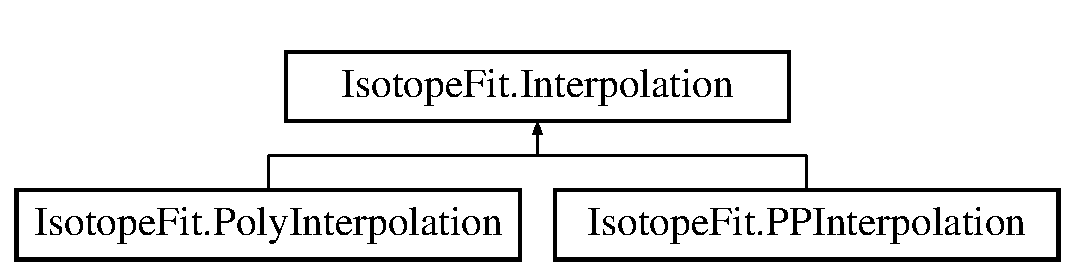
\includegraphics[height=2.000000cm]{class_isotope_fit_1_1_interpolation}
\end{center}
\end{figure}
\subsection*{Classes}
\begin{DoxyCompactItemize}
\item 
class \mbox{\hyperlink{class_isotope_fit_1_1_interpolation_1_1_interpolation_exception}{Interpolation\+Exception}}
\end{DoxyCompactItemize}
\subsection*{Public Types}
\begin{DoxyCompactItemize}
\item 
\mbox{\Hypertarget{class_isotope_fit_1_1_interpolation_af374d540896ff406c38322a30a4477b4}\label{class_isotope_fit_1_1_interpolation_af374d540896ff406c38322a30a4477b4}} 
enum {\bfseries Type} \{ {\bfseries Polynomial}, 
{\bfseries Spline\+Natural}, 
{\bfseries Spline\+Not\+A\+Knot}, 
{\bfseries P\+C\+H\+IP}
 \}
\end{DoxyCompactItemize}
\subsection*{Public Member Functions}
\begin{DoxyCompactItemize}
\item 
\mbox{\Hypertarget{class_isotope_fit_1_1_interpolation_ac9c7f5985c6f956e03db0b0de233d514}\label{class_isotope_fit_1_1_interpolation_ac9c7f5985c6f956e03db0b0de233d514}} 
abstract double {\bfseries Evaluate} (double x)
\item 
\mbox{\Hypertarget{class_isotope_fit_1_1_interpolation_afe9c495f3e3eae57b1019428f7f70192}\label{class_isotope_fit_1_1_interpolation_afe9c495f3e3eae57b1019428f7f70192}} 
abstract double \mbox{[}$\,$\mbox{]} {\bfseries Evaluate} (double\mbox{[}$\,$\mbox{]} x)
\end{DoxyCompactItemize}
\subsection*{Protected Attributes}
\begin{DoxyCompactItemize}
\item 
\mbox{\Hypertarget{class_isotope_fit_1_1_interpolation_acf6347fae287029b998501472537d0a4}\label{class_isotope_fit_1_1_interpolation_acf6347fae287029b998501472537d0a4}} 
double \mbox{[}$\,$\mbox{]} {\bfseries x\+Values}
\item 
\mbox{\Hypertarget{class_isotope_fit_1_1_interpolation_adaf07c17ecb29957a3daf18b35947468}\label{class_isotope_fit_1_1_interpolation_adaf07c17ecb29957a3daf18b35947468}} 
double \mbox{[}$\,$\mbox{]} {\bfseries y\+Values}
\end{DoxyCompactItemize}


\subsection{Detailed Description}
Base class that handles data interpolations and related data. 



Definition at line 12 of file Interpolation.\+cs.



The documentation for this class was generated from the following file\+:\begin{DoxyCompactItemize}
\item 
Isotope\+Fit\+Lib/\+Numerics/Interpolation.\+cs\end{DoxyCompactItemize}

\hypertarget{class_isotope_fit_1_1_interpolation_1_1_interpolation_exception}{}\section{Isotope\+Fit.\+Interpolation.\+Interpolation\+Exception Class Reference}
\label{class_isotope_fit_1_1_interpolation_1_1_interpolation_exception}\index{Isotope\+Fit.\+Interpolation.\+Interpolation\+Exception@{Isotope\+Fit.\+Interpolation.\+Interpolation\+Exception}}
Inheritance diagram for Isotope\+Fit.\+Interpolation.\+Interpolation\+Exception\+:\begin{figure}[H]
\begin{center}
\leavevmode
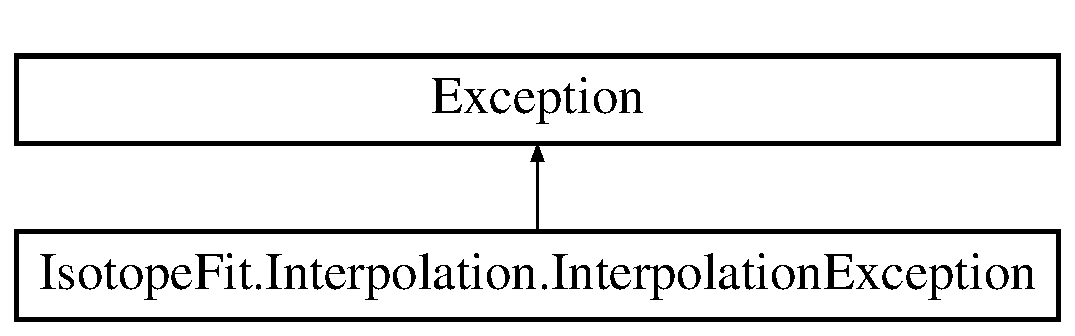
\includegraphics[height=2.000000cm]{class_isotope_fit_1_1_interpolation_1_1_interpolation_exception}
\end{center}
\end{figure}
\subsection*{Public Member Functions}
\begin{DoxyCompactItemize}
\item 
\mbox{\Hypertarget{class_isotope_fit_1_1_interpolation_1_1_interpolation_exception_a9e94ab620a10ae4086570d04c3487bca}\label{class_isotope_fit_1_1_interpolation_1_1_interpolation_exception_a9e94ab620a10ae4086570d04c3487bca}} 
{\bfseries Interpolation\+Exception} (string message)
\item 
\mbox{\Hypertarget{class_isotope_fit_1_1_interpolation_1_1_interpolation_exception_aa3d1266e6b875169acec315c043c5d50}\label{class_isotope_fit_1_1_interpolation_1_1_interpolation_exception_aa3d1266e6b875169acec315c043c5d50}} 
{\bfseries Interpolation\+Exception} (string message, Exception inner)
\end{DoxyCompactItemize}
\subsection*{Protected Member Functions}
\begin{DoxyCompactItemize}
\item 
\mbox{\Hypertarget{class_isotope_fit_1_1_interpolation_1_1_interpolation_exception_a1580559b679fda8e19fa66cad9886440}\label{class_isotope_fit_1_1_interpolation_1_1_interpolation_exception_a1580559b679fda8e19fa66cad9886440}} 
{\bfseries Interpolation\+Exception} (System.\+Runtime.\+Serialization.\+Serialization\+Info info, System.\+Runtime.\+Serialization.\+Streaming\+Context context)
\end{DoxyCompactItemize}


\subsection{Detailed Description}


Definition at line 29 of file Interpolation.\+cs.



The documentation for this class was generated from the following file\+:\begin{DoxyCompactItemize}
\item 
Isotope\+Fit\+Lib/\+Numerics/Interpolation.\+cs\end{DoxyCompactItemize}

\hypertarget{class_isotope_fit_1_1_i_f_data_1_1_cluster_1_1_isotope_data}{}\section{Isotope\+Fit.\+I\+F\+Data.\+Cluster.\+Isotope\+Data Class Reference}
\label{class_isotope_fit_1_1_i_f_data_1_1_cluster_1_1_isotope_data}\index{Isotope\+Fit.\+I\+F\+Data.\+Cluster.\+Isotope\+Data@{Isotope\+Fit.\+I\+F\+Data.\+Cluster.\+Isotope\+Data}}


Class to store data about the isotopical pattern of a molecule/fragment.  


\subsection*{Properties}
\begin{DoxyCompactItemize}
\item 
\mbox{\Hypertarget{class_isotope_fit_1_1_i_f_data_1_1_cluster_1_1_isotope_data_afbbe848f60b456135ea622abf0644d1b}\label{class_isotope_fit_1_1_i_f_data_1_1_cluster_1_1_isotope_data_afbbe848f60b456135ea622abf0644d1b}} 
double \mbox{[}$\,$\mbox{]} {\bfseries Mass}\hspace{0.3cm}{\ttfamily  \mbox{[}get, set\mbox{]}}
\item 
\mbox{\Hypertarget{class_isotope_fit_1_1_i_f_data_1_1_cluster_1_1_isotope_data_aa0f17487c627ed87bedc9cbd2670fc09}\label{class_isotope_fit_1_1_i_f_data_1_1_cluster_1_1_isotope_data_aa0f17487c627ed87bedc9cbd2670fc09}} 
double \mbox{[}$\,$\mbox{]} {\bfseries Abundance}\hspace{0.3cm}{\ttfamily  \mbox{[}get, set\mbox{]}}
\end{DoxyCompactItemize}


\subsection{Detailed Description}
Class to store data about the isotopical pattern of a molecule/fragment. 



Definition at line 186 of file I\+F\+Data.\+cs.



The documentation for this class was generated from the following file\+:\begin{DoxyCompactItemize}
\item 
Isotope\+Fit\+Lib/I\+F\+Data.\+cs\end{DoxyCompactItemize}

\hypertarget{class_isotope_fit_1_1_least_squares_system}{}\section{Isotope\+Fit.\+Least\+Squares\+System Class Reference}
\label{class_isotope_fit_1_1_least_squares_system}\index{Isotope\+Fit.\+Least\+Squares\+System@{Isotope\+Fit.\+Least\+Squares\+System}}


Class for handling least squares systems.  


\subsection*{Public Member Functions}
\begin{DoxyCompactItemize}
\item 
\hyperlink{class_isotope_fit_1_1_least_squares_system_aec0b3973e7239d006b752a4e079f80d0}{Least\+Squares\+System} (Sparse\+Matrix des\+Mat, Vector$<$ double $>$ obs\+Vec)
\begin{DoxyCompactList}\small\item\em Creates new least squares system and populates it with the supplied data. \end{DoxyCompactList}\item 
void \hyperlink{class_isotope_fit_1_1_least_squares_system_ac72b8568e9ecb97077102658f56aba3f}{Solve} ()
\begin{DoxyCompactList}\small\item\em Calls the least square solver method and stores the result in the Solution property. \end{DoxyCompactList}\end{DoxyCompactItemize}
\subsection*{Properties}
\begin{DoxyCompactItemize}
\item 
\mbox{\Hypertarget{class_isotope_fit_1_1_least_squares_system_a843dc1bf5e21d7a6a6ac9d5339386f92}\label{class_isotope_fit_1_1_least_squares_system_a843dc1bf5e21d7a6a6ac9d5339386f92}} 
Vector$<$ double $>$ {\bfseries Solution}\hspace{0.3cm}{\ttfamily  \mbox{[}get\mbox{]}}
\end{DoxyCompactItemize}


\subsection{Detailed Description}
Class for handling least squares systems. 



Definition at line 17 of file Least\+Squares\+System.\+cs.



\subsection{Constructor \& Destructor Documentation}
\mbox{\Hypertarget{class_isotope_fit_1_1_least_squares_system_aec0b3973e7239d006b752a4e079f80d0}\label{class_isotope_fit_1_1_least_squares_system_aec0b3973e7239d006b752a4e079f80d0}} 
\index{Isotope\+Fit\+::\+Least\+Squares\+System@{Isotope\+Fit\+::\+Least\+Squares\+System}!Least\+Squares\+System@{Least\+Squares\+System}}
\index{Least\+Squares\+System@{Least\+Squares\+System}!Isotope\+Fit\+::\+Least\+Squares\+System@{Isotope\+Fit\+::\+Least\+Squares\+System}}
\subsubsection{\texorpdfstring{Least\+Squares\+System()}{LeastSquaresSystem()}}
{\footnotesize\ttfamily Isotope\+Fit.\+Least\+Squares\+System.\+Least\+Squares\+System (\begin{DoxyParamCaption}\item[{Sparse\+Matrix}]{des\+Mat,  }\item[{Vector$<$ double $>$}]{obs\+Vec }\end{DoxyParamCaption})}



Creates new least squares system and populates it with the supplied data. 


\begin{DoxyParams}{Parameters}
{\em des\+Mat} & Design matrix of the least squares system.\\
\hline
{\em obs\+Vec} & Vector of observations of the least squares system.\\
\hline
\end{DoxyParams}


Definition at line 24 of file Least\+Squares\+System.\+cs.



\subsection{Member Function Documentation}
\mbox{\Hypertarget{class_isotope_fit_1_1_least_squares_system_ac72b8568e9ecb97077102658f56aba3f}\label{class_isotope_fit_1_1_least_squares_system_ac72b8568e9ecb97077102658f56aba3f}} 
\index{Isotope\+Fit\+::\+Least\+Squares\+System@{Isotope\+Fit\+::\+Least\+Squares\+System}!Solve@{Solve}}
\index{Solve@{Solve}!Isotope\+Fit\+::\+Least\+Squares\+System@{Isotope\+Fit\+::\+Least\+Squares\+System}}
\subsubsection{\texorpdfstring{Solve()}{Solve()}}
{\footnotesize\ttfamily void Isotope\+Fit.\+Least\+Squares\+System.\+Solve (\begin{DoxyParamCaption}{ }\end{DoxyParamCaption})}



Calls the least square solver method and stores the result in the Solution property. 

At the moment, only non-\/negative least squares solver is implemented. 

Definition at line 41 of file Least\+Squares\+System.\+cs.



The documentation for this class was generated from the following file\+:\begin{DoxyCompactItemize}
\item 
Isotope\+Fit\+Lib/\+Numerics/Least\+Squares\+System.\+cs\end{DoxyCompactItemize}

\hypertarget{class_isotope_fit_1_1_i_f_data_1_1_calibration_1_1_line_shape}{}\section{Isotope\+Fit.\+I\+F\+Data.\+Calibration.\+Line\+Shape Class Reference}
\label{class_isotope_fit_1_1_i_f_data_1_1_calibration_1_1_line_shape}\index{Isotope\+Fit.\+I\+F\+Data.\+Calibration.\+Line\+Shape@{Isotope\+Fit.\+I\+F\+Data.\+Calibration.\+Line\+Shape}}


Class containing the information about line shape.  


\subsection*{Public Member Functions}
\begin{DoxyCompactItemize}
\item 
\mbox{\Hypertarget{class_isotope_fit_1_1_i_f_data_1_1_calibration_1_1_line_shape_ab5ed4d295ead4741f309d80fee17addc}\label{class_isotope_fit_1_1_i_f_data_1_1_calibration_1_1_line_shape_ab5ed4d295ead4741f309d80fee17addc}} 
{\bfseries Line\+Shape} (double\mbox{[}$\,$\mbox{]} breaks, double\mbox{[}$\,$\mbox{]}\mbox{[}$\,$\mbox{]} coeffs)
\end{DoxyCompactItemize}
\subsection*{Properties}
\begin{DoxyCompactItemize}
\item 
double \mbox{[}$\,$\mbox{]} \hyperlink{class_isotope_fit_1_1_i_f_data_1_1_calibration_1_1_line_shape_a447511120da7a7c67677aeb723cffd77}{Breaks}\hspace{0.3cm}{\ttfamily  \mbox{[}get, set\mbox{]}}
\begin{DoxyCompactList}\small\item\em Breaks of the partial polynomial describing the line shape \end{DoxyCompactList}\item 
Matrix$<$ double $>$ \hyperlink{class_isotope_fit_1_1_i_f_data_1_1_calibration_1_1_line_shape_a8892e37963113bc557f3324a10ff82a0}{Coeffs}\hspace{0.3cm}{\ttfamily  \mbox{[}get, set\mbox{]}}
\begin{DoxyCompactList}\small\item\em Coefficients of the partial polynomial describing the line shape \end{DoxyCompactList}\end{DoxyCompactItemize}


\subsection{Detailed Description}
Class containing the information about line shape. 



Definition at line 339 of file I\+F\+Data.\+cs.



\subsection{Property Documentation}
\mbox{\Hypertarget{class_isotope_fit_1_1_i_f_data_1_1_calibration_1_1_line_shape_a447511120da7a7c67677aeb723cffd77}\label{class_isotope_fit_1_1_i_f_data_1_1_calibration_1_1_line_shape_a447511120da7a7c67677aeb723cffd77}} 
\index{Isotope\+Fit\+::\+I\+F\+Data\+::\+Calibration\+::\+Line\+Shape@{Isotope\+Fit\+::\+I\+F\+Data\+::\+Calibration\+::\+Line\+Shape}!Breaks@{Breaks}}
\index{Breaks@{Breaks}!Isotope\+Fit\+::\+I\+F\+Data\+::\+Calibration\+::\+Line\+Shape@{Isotope\+Fit\+::\+I\+F\+Data\+::\+Calibration\+::\+Line\+Shape}}
\subsubsection{\texorpdfstring{Breaks}{Breaks}}
{\footnotesize\ttfamily double \mbox{[}$\,$\mbox{]} Isotope\+Fit.\+I\+F\+Data.\+Calibration.\+Line\+Shape.\+Breaks\hspace{0.3cm}{\ttfamily [get]}, {\ttfamily [set]}}



Breaks of the partial polynomial describing the line shape 



Definition at line 354 of file I\+F\+Data.\+cs.

\mbox{\Hypertarget{class_isotope_fit_1_1_i_f_data_1_1_calibration_1_1_line_shape_a8892e37963113bc557f3324a10ff82a0}\label{class_isotope_fit_1_1_i_f_data_1_1_calibration_1_1_line_shape_a8892e37963113bc557f3324a10ff82a0}} 
\index{Isotope\+Fit\+::\+I\+F\+Data\+::\+Calibration\+::\+Line\+Shape@{Isotope\+Fit\+::\+I\+F\+Data\+::\+Calibration\+::\+Line\+Shape}!Coeffs@{Coeffs}}
\index{Coeffs@{Coeffs}!Isotope\+Fit\+::\+I\+F\+Data\+::\+Calibration\+::\+Line\+Shape@{Isotope\+Fit\+::\+I\+F\+Data\+::\+Calibration\+::\+Line\+Shape}}
\subsubsection{\texorpdfstring{Coeffs}{Coeffs}}
{\footnotesize\ttfamily Matrix$<$double$>$ Isotope\+Fit.\+I\+F\+Data.\+Calibration.\+Line\+Shape.\+Coeffs\hspace{0.3cm}{\ttfamily [get]}, {\ttfamily [set]}}



Coefficients of the partial polynomial describing the line shape 



Definition at line 359 of file I\+F\+Data.\+cs.



The documentation for this class was generated from the following file\+:\begin{DoxyCompactItemize}
\item 
Isotope\+Fit\+Lib/I\+F\+Data.\+cs\end{DoxyCompactItemize}

\hypertarget{class_isotope_fit_1_1_poly_interpolation}{}\section{Isotope\+Fit.\+Poly\+Interpolation Class Reference}
\label{class_isotope_fit_1_1_poly_interpolation}\index{Isotope\+Fit.\+Poly\+Interpolation@{Isotope\+Fit.\+Poly\+Interpolation}}


Derived class that handles polynomial interpolations and evaluation of data.  


Inheritance diagram for Isotope\+Fit.\+Poly\+Interpolation\+:\begin{figure}[H]
\begin{center}
\leavevmode
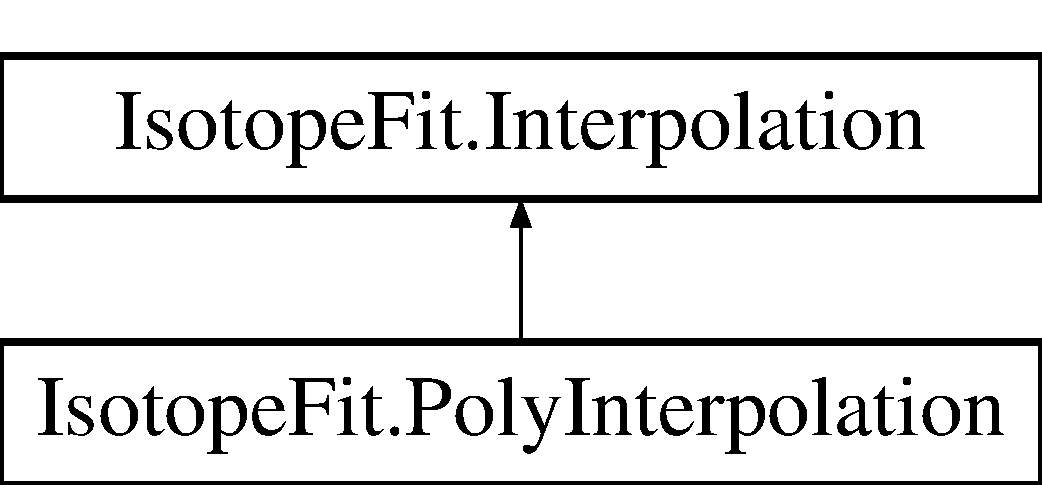
\includegraphics[height=2.000000cm]{class_isotope_fit_1_1_poly_interpolation}
\end{center}
\end{figure}
\subsection*{Public Member Functions}
\begin{DoxyCompactItemize}
\item 
\mbox{\hyperlink{class_isotope_fit_1_1_poly_interpolation_a0ad4d407eb80baf6c38b3b752048e285}{Poly\+Interpolation}} (double\mbox{[}$\,$\mbox{]} x, double\mbox{[}$\,$\mbox{]} y, int order)
\begin{DoxyCompactList}\small\item\em Creates new interpolation object and calculates polynomial interpolation parameters. \end{DoxyCompactList}\item 
\mbox{\hyperlink{class_isotope_fit_1_1_poly_interpolation_afb26a6b07ac8ca8fb710682c437f6d7f}{Poly\+Interpolation}} (double\mbox{[}$\,$\mbox{]} coefs)
\begin{DoxyCompactList}\small\item\em Creates new interpolation object and stores already known interpolation coeficients. \end{DoxyCompactList}\item 
override double \mbox{\hyperlink{class_isotope_fit_1_1_poly_interpolation_a9638e5613d8a6537b73db6fe37ccd9e8}{Evaluate}} (double x)
\begin{DoxyCompactList}\small\item\em Initializes a polynomial evaluation of a selected point x. \end{DoxyCompactList}\item 
override double \mbox{[}$\,$\mbox{]} \mbox{\hyperlink{class_isotope_fit_1_1_poly_interpolation_ad6c5b40f7a718d934c5a3ed7f55c5eb3}{Evaluate}} (double\mbox{[}$\,$\mbox{]} x)
\begin{DoxyCompactList}\small\item\em Initializes a polynomial evaluation of a selected array of points x. \end{DoxyCompactList}\end{DoxyCompactItemize}
\subsection*{Properties}
\begin{DoxyCompactItemize}
\item 
\mbox{\Hypertarget{class_isotope_fit_1_1_poly_interpolation_a15443a5303b14cf3a4257209c356d5d8}\label{class_isotope_fit_1_1_poly_interpolation_a15443a5303b14cf3a4257209c356d5d8}} 
double \mbox{[}$\,$\mbox{]} {\bfseries Coefs}\hspace{0.3cm}{\ttfamily  \mbox{[}get\mbox{]}}
\item 
\mbox{\Hypertarget{class_isotope_fit_1_1_poly_interpolation_a9145d70d1259efee946f5deed75666d8}\label{class_isotope_fit_1_1_poly_interpolation_a9145d70d1259efee946f5deed75666d8}} 
int {\bfseries Order}\hspace{0.3cm}{\ttfamily  \mbox{[}get\mbox{]}}
\end{DoxyCompactItemize}
\subsection*{Additional Inherited Members}


\subsection{Detailed Description}
Derived class that handles polynomial interpolations and evaluation of data. 



Definition at line 15 of file Poly\+Interpolation.\+cs.



\subsection{Constructor \& Destructor Documentation}
\mbox{\Hypertarget{class_isotope_fit_1_1_poly_interpolation_a0ad4d407eb80baf6c38b3b752048e285}\label{class_isotope_fit_1_1_poly_interpolation_a0ad4d407eb80baf6c38b3b752048e285}} 
\index{Isotope\+Fit\+::\+Poly\+Interpolation@{Isotope\+Fit\+::\+Poly\+Interpolation}!Poly\+Interpolation@{Poly\+Interpolation}}
\index{Poly\+Interpolation@{Poly\+Interpolation}!Isotope\+Fit\+::\+Poly\+Interpolation@{Isotope\+Fit\+::\+Poly\+Interpolation}}
\subsubsection{\texorpdfstring{Poly\+Interpolation()}{PolyInterpolation()}\hspace{0.1cm}{\footnotesize\ttfamily [1/2]}}
{\footnotesize\ttfamily Isotope\+Fit.\+Poly\+Interpolation.\+Poly\+Interpolation (\begin{DoxyParamCaption}\item[{double \mbox{[}$\,$\mbox{]}}]{x,  }\item[{double \mbox{[}$\,$\mbox{]}}]{y,  }\item[{int}]{order }\end{DoxyParamCaption})}



Creates new interpolation object and calculates polynomial interpolation parameters. 


\begin{DoxyParams}{Parameters}
{\em x} & Array of x values.\\
\hline
{\em y} & Array of y values.\\
\hline
{\em order} & Order of polynomial.\\
\hline
\end{DoxyParams}


Definition at line 25 of file Poly\+Interpolation.\+cs.

\mbox{\Hypertarget{class_isotope_fit_1_1_poly_interpolation_afb26a6b07ac8ca8fb710682c437f6d7f}\label{class_isotope_fit_1_1_poly_interpolation_afb26a6b07ac8ca8fb710682c437f6d7f}} 
\index{Isotope\+Fit\+::\+Poly\+Interpolation@{Isotope\+Fit\+::\+Poly\+Interpolation}!Poly\+Interpolation@{Poly\+Interpolation}}
\index{Poly\+Interpolation@{Poly\+Interpolation}!Isotope\+Fit\+::\+Poly\+Interpolation@{Isotope\+Fit\+::\+Poly\+Interpolation}}
\subsubsection{\texorpdfstring{Poly\+Interpolation()}{PolyInterpolation()}\hspace{0.1cm}{\footnotesize\ttfamily [2/2]}}
{\footnotesize\ttfamily Isotope\+Fit.\+Poly\+Interpolation.\+Poly\+Interpolation (\begin{DoxyParamCaption}\item[{double \mbox{[}$\,$\mbox{]}}]{coefs }\end{DoxyParamCaption})}



Creates new interpolation object and stores already known interpolation coeficients. 

Input polynomial coefficients have to be sorted by increasing power from left to right in array. 


\begin{DoxyParams}{Parameters}
{\em coefs} & Array of polynomial coefficients.\\
\hline
\end{DoxyParams}


Definition at line 47 of file Poly\+Interpolation.\+cs.



\subsection{Member Function Documentation}
\mbox{\Hypertarget{class_isotope_fit_1_1_poly_interpolation_a9638e5613d8a6537b73db6fe37ccd9e8}\label{class_isotope_fit_1_1_poly_interpolation_a9638e5613d8a6537b73db6fe37ccd9e8}} 
\index{Isotope\+Fit\+::\+Poly\+Interpolation@{Isotope\+Fit\+::\+Poly\+Interpolation}!Evaluate@{Evaluate}}
\index{Evaluate@{Evaluate}!Isotope\+Fit\+::\+Poly\+Interpolation@{Isotope\+Fit\+::\+Poly\+Interpolation}}
\subsubsection{\texorpdfstring{Evaluate()}{Evaluate()}\hspace{0.1cm}{\footnotesize\ttfamily [1/2]}}
{\footnotesize\ttfamily override double Isotope\+Fit.\+Poly\+Interpolation.\+Evaluate (\begin{DoxyParamCaption}\item[{double}]{x }\end{DoxyParamCaption})\hspace{0.3cm}{\ttfamily [virtual]}}



Initializes a polynomial evaluation of a selected point x. 


\begin{DoxyParams}{Parameters}
{\em x} & Single x value.\\
\hline
\end{DoxyParams}
\begin{DoxyReturn}{Returns}
Single evaluated y value.
\end{DoxyReturn}


Implements \mbox{\hyperlink{class_isotope_fit_1_1_interpolation}{Isotope\+Fit.\+Interpolation}}.



Definition at line 80 of file Poly\+Interpolation.\+cs.

\mbox{\Hypertarget{class_isotope_fit_1_1_poly_interpolation_ad6c5b40f7a718d934c5a3ed7f55c5eb3}\label{class_isotope_fit_1_1_poly_interpolation_ad6c5b40f7a718d934c5a3ed7f55c5eb3}} 
\index{Isotope\+Fit\+::\+Poly\+Interpolation@{Isotope\+Fit\+::\+Poly\+Interpolation}!Evaluate@{Evaluate}}
\index{Evaluate@{Evaluate}!Isotope\+Fit\+::\+Poly\+Interpolation@{Isotope\+Fit\+::\+Poly\+Interpolation}}
\subsubsection{\texorpdfstring{Evaluate()}{Evaluate()}\hspace{0.1cm}{\footnotesize\ttfamily [2/2]}}
{\footnotesize\ttfamily override double \mbox{[}$\,$\mbox{]} Isotope\+Fit.\+Poly\+Interpolation.\+Evaluate (\begin{DoxyParamCaption}\item[{double \mbox{[}$\,$\mbox{]}}]{x }\end{DoxyParamCaption})\hspace{0.3cm}{\ttfamily [virtual]}}



Initializes a polynomial evaluation of a selected array of points x. 


\begin{DoxyParams}{Parameters}
{\em x} & Array of x values.\\
\hline
\end{DoxyParams}
\begin{DoxyReturn}{Returns}
Array of evaluated y values.
\end{DoxyReturn}


Implements \mbox{\hyperlink{class_isotope_fit_1_1_interpolation}{Isotope\+Fit.\+Interpolation}}.



Definition at line 90 of file Poly\+Interpolation.\+cs.



The documentation for this class was generated from the following file\+:\begin{DoxyCompactItemize}
\item 
Isotope\+Fit\+Lib/\+Numerics/Poly\+Interpolation.\+cs\end{DoxyCompactItemize}

\hypertarget{class_isotope_fit_1_1_p_p_interpolation}{}\section{Isotope\+Fit.\+P\+P\+Interpolation Class Reference}
\label{class_isotope_fit_1_1_p_p_interpolation}\index{Isotope\+Fit.\+P\+P\+Interpolation@{Isotope\+Fit.\+P\+P\+Interpolation}}


Derived class that handles piecewise polynomial interpolations and evaluation of data.  


Inheritance diagram for Isotope\+Fit.\+P\+P\+Interpolation\+:\begin{figure}[H]
\begin{center}
\leavevmode
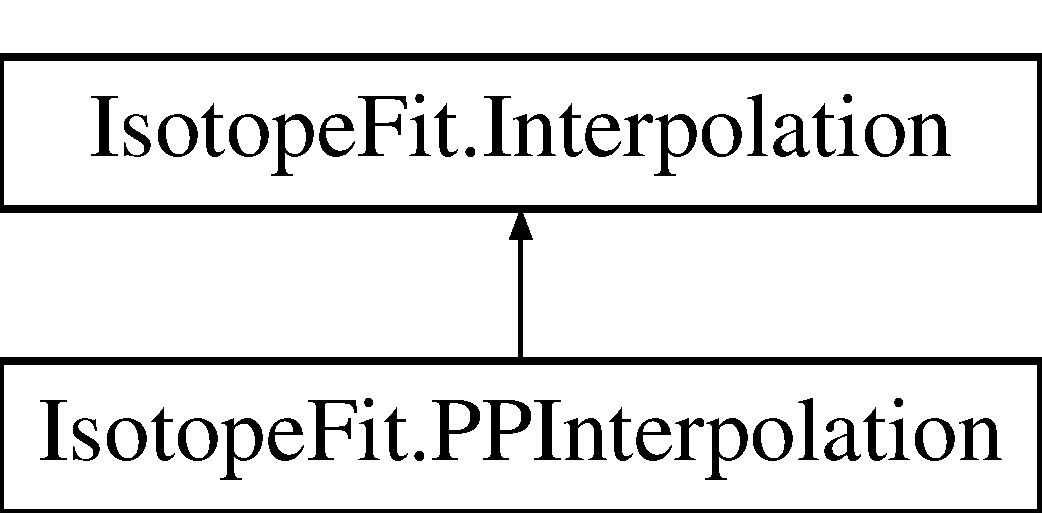
\includegraphics[height=2.000000cm]{class_isotope_fit_1_1_p_p_interpolation}
\end{center}
\end{figure}
\subsection*{Public Types}
\begin{DoxyCompactItemize}
\item 
\mbox{\Hypertarget{class_isotope_fit_1_1_p_p_interpolation_ab16ae4c5036a290c4db168e75973ff1e}\label{class_isotope_fit_1_1_p_p_interpolation_ab16ae4c5036a290c4db168e75973ff1e}} 
enum {\bfseries P\+P\+Type} \{ {\bfseries Spline\+Natural}, 
{\bfseries Spline\+Not\+A\+Knot}, 
{\bfseries P\+C\+H\+IP}
 \}
\end{DoxyCompactItemize}
\subsection*{Public Member Functions}
\begin{DoxyCompactItemize}
\item 
\mbox{\hyperlink{class_isotope_fit_1_1_p_p_interpolation_afaeb635a338f06714d3b12e3865ac4f2}{P\+P\+Interpolation}} (double\mbox{[}$\,$\mbox{]} x, double\mbox{[}$\,$\mbox{]} y, P\+P\+Type t)
\begin{DoxyCompactList}\small\item\em Creates new interpolation object and calculates piecewise polynomial interpolation parameters. \end{DoxyCompactList}\item 
\mbox{\hyperlink{class_isotope_fit_1_1_p_p_interpolation_a22298333495a707643412a540e461188}{P\+P\+Interpolation}} (double\mbox{[}$\,$\mbox{]} breaks, double\mbox{[}$\,$\mbox{]}\mbox{[}$\,$\mbox{]} coefs)
\begin{DoxyCompactList}\small\item\em Creates new interpolation object and stores already known interpolation parameters. \end{DoxyCompactList}\item 
override double \mbox{\hyperlink{class_isotope_fit_1_1_p_p_interpolation_a1849081f6f187cb948c7f8f7dba866af}{Evaluate}} (double x)
\begin{DoxyCompactList}\small\item\em Initializes a piecewise cubic polynomial evaluation of a selected point x. \end{DoxyCompactList}\item 
override double \mbox{[}$\,$\mbox{]} \mbox{\hyperlink{class_isotope_fit_1_1_p_p_interpolation_a5a4a1dbfcaa78e520dfc965e64ed227c}{Evaluate}} (double\mbox{[}$\,$\mbox{]} x)
\begin{DoxyCompactList}\small\item\em Initializes a piecewise cubic polynomial evaluation of a selected array of points x. \end{DoxyCompactList}\end{DoxyCompactItemize}
\subsection*{Properties}
\begin{DoxyCompactItemize}
\item 
\mbox{\Hypertarget{class_isotope_fit_1_1_p_p_interpolation_a0e77da81cfa5f6377e81d5855ee82a32}\label{class_isotope_fit_1_1_p_p_interpolation_a0e77da81cfa5f6377e81d5855ee82a32}} 
P\+P\+Type {\bfseries pp\+Type}\hspace{0.3cm}{\ttfamily  \mbox{[}get\mbox{]}}
\item 
\mbox{\Hypertarget{class_isotope_fit_1_1_p_p_interpolation_ac9ccf388cee3f262e6db2c6ba757429d}\label{class_isotope_fit_1_1_p_p_interpolation_ac9ccf388cee3f262e6db2c6ba757429d}} 
double \mbox{[}$\,$\mbox{]} {\bfseries Breaks}\hspace{0.3cm}{\ttfamily  \mbox{[}get\mbox{]}}
\item 
\mbox{\Hypertarget{class_isotope_fit_1_1_p_p_interpolation_ae7548d6f546a8b4ac1b1d6f4e70d7819}\label{class_isotope_fit_1_1_p_p_interpolation_ae7548d6f546a8b4ac1b1d6f4e70d7819}} 
double \mbox{[}$\,$\mbox{]}\mbox{[}$\,$\mbox{]} {\bfseries Coefs}\hspace{0.3cm}{\ttfamily  \mbox{[}get\mbox{]}}
\end{DoxyCompactItemize}
\subsection*{Additional Inherited Members}


\subsection{Detailed Description}
Derived class that handles piecewise polynomial interpolations and evaluation of data. 



Definition at line 17 of file P\+P\+Interpolation.\+cs.



\subsection{Constructor \& Destructor Documentation}
\mbox{\Hypertarget{class_isotope_fit_1_1_p_p_interpolation_afaeb635a338f06714d3b12e3865ac4f2}\label{class_isotope_fit_1_1_p_p_interpolation_afaeb635a338f06714d3b12e3865ac4f2}} 
\index{Isotope\+Fit\+::\+P\+P\+Interpolation@{Isotope\+Fit\+::\+P\+P\+Interpolation}!P\+P\+Interpolation@{P\+P\+Interpolation}}
\index{P\+P\+Interpolation@{P\+P\+Interpolation}!Isotope\+Fit\+::\+P\+P\+Interpolation@{Isotope\+Fit\+::\+P\+P\+Interpolation}}
\subsubsection{\texorpdfstring{P\+P\+Interpolation()}{PPInterpolation()}\hspace{0.1cm}{\footnotesize\ttfamily [1/2]}}
{\footnotesize\ttfamily Isotope\+Fit.\+P\+P\+Interpolation.\+P\+P\+Interpolation (\begin{DoxyParamCaption}\item[{double \mbox{[}$\,$\mbox{]}}]{x,  }\item[{double \mbox{[}$\,$\mbox{]}}]{y,  }\item[{P\+P\+Type}]{t }\end{DoxyParamCaption})}



Creates new interpolation object and calculates piecewise polynomial interpolation parameters. 


\begin{DoxyParams}{Parameters}
{\em x} & Array of x values.\\
\hline
{\em y} & Array of y values.\\
\hline
{\em t} & Piecewise polynomial interpolation type.\\
\hline
\end{DoxyParams}


Definition at line 27 of file P\+P\+Interpolation.\+cs.

\mbox{\Hypertarget{class_isotope_fit_1_1_p_p_interpolation_a22298333495a707643412a540e461188}\label{class_isotope_fit_1_1_p_p_interpolation_a22298333495a707643412a540e461188}} 
\index{Isotope\+Fit\+::\+P\+P\+Interpolation@{Isotope\+Fit\+::\+P\+P\+Interpolation}!P\+P\+Interpolation@{P\+P\+Interpolation}}
\index{P\+P\+Interpolation@{P\+P\+Interpolation}!Isotope\+Fit\+::\+P\+P\+Interpolation@{Isotope\+Fit\+::\+P\+P\+Interpolation}}
\subsubsection{\texorpdfstring{P\+P\+Interpolation()}{PPInterpolation()}\hspace{0.1cm}{\footnotesize\ttfamily [2/2]}}
{\footnotesize\ttfamily Isotope\+Fit.\+P\+P\+Interpolation.\+P\+P\+Interpolation (\begin{DoxyParamCaption}\item[{double \mbox{[}$\,$\mbox{]}}]{breaks,  }\item[{double}]{coefs\mbox{[}$\,$\mbox{]}\mbox{[}$\,$\mbox{]} }\end{DoxyParamCaption})}



Creates new interpolation object and stores already known interpolation parameters. 

Input polynomial coefficients have to be sorted by increasing power from left to right in 2D array. 


\begin{DoxyParams}{Parameters}
{\em breaks} & Array of break points.\\
\hline
{\em coefs} & 2D array of polynomial coefficients.\\
\hline
\end{DoxyParams}


Definition at line 44 of file P\+P\+Interpolation.\+cs.



\subsection{Member Function Documentation}
\mbox{\Hypertarget{class_isotope_fit_1_1_p_p_interpolation_a1849081f6f187cb948c7f8f7dba866af}\label{class_isotope_fit_1_1_p_p_interpolation_a1849081f6f187cb948c7f8f7dba866af}} 
\index{Isotope\+Fit\+::\+P\+P\+Interpolation@{Isotope\+Fit\+::\+P\+P\+Interpolation}!Evaluate@{Evaluate}}
\index{Evaluate@{Evaluate}!Isotope\+Fit\+::\+P\+P\+Interpolation@{Isotope\+Fit\+::\+P\+P\+Interpolation}}
\subsubsection{\texorpdfstring{Evaluate()}{Evaluate()}\hspace{0.1cm}{\footnotesize\ttfamily [1/2]}}
{\footnotesize\ttfamily override double Isotope\+Fit.\+P\+P\+Interpolation.\+Evaluate (\begin{DoxyParamCaption}\item[{double}]{x }\end{DoxyParamCaption})\hspace{0.3cm}{\ttfamily [virtual]}}



Initializes a piecewise cubic polynomial evaluation of a selected point x. 


\begin{DoxyParams}{Parameters}
{\em x} & Single x value.\\
\hline
\end{DoxyParams}
\begin{DoxyReturn}{Returns}
Single evaluated y value.
\end{DoxyReturn}


Implements \mbox{\hyperlink{class_isotope_fit_1_1_interpolation}{Isotope\+Fit.\+Interpolation}}.



Definition at line 311 of file P\+P\+Interpolation.\+cs.

\mbox{\Hypertarget{class_isotope_fit_1_1_p_p_interpolation_a5a4a1dbfcaa78e520dfc965e64ed227c}\label{class_isotope_fit_1_1_p_p_interpolation_a5a4a1dbfcaa78e520dfc965e64ed227c}} 
\index{Isotope\+Fit\+::\+P\+P\+Interpolation@{Isotope\+Fit\+::\+P\+P\+Interpolation}!Evaluate@{Evaluate}}
\index{Evaluate@{Evaluate}!Isotope\+Fit\+::\+P\+P\+Interpolation@{Isotope\+Fit\+::\+P\+P\+Interpolation}}
\subsubsection{\texorpdfstring{Evaluate()}{Evaluate()}\hspace{0.1cm}{\footnotesize\ttfamily [2/2]}}
{\footnotesize\ttfamily override double \mbox{[}$\,$\mbox{]} Isotope\+Fit.\+P\+P\+Interpolation.\+Evaluate (\begin{DoxyParamCaption}\item[{double \mbox{[}$\,$\mbox{]}}]{x }\end{DoxyParamCaption})\hspace{0.3cm}{\ttfamily [virtual]}}



Initializes a piecewise cubic polynomial evaluation of a selected array of points x. 


\begin{DoxyParams}{Parameters}
{\em x} & Array of x values.\\
\hline
\end{DoxyParams}
\begin{DoxyReturn}{Returns}
Array of evaluated y values.
\end{DoxyReturn}


Implements \mbox{\hyperlink{class_isotope_fit_1_1_interpolation}{Isotope\+Fit.\+Interpolation}}.



Definition at line 321 of file P\+P\+Interpolation.\+cs.



The documentation for this class was generated from the following file\+:\begin{DoxyCompactItemize}
\item 
Isotope\+Fit\+Lib/\+Numerics/P\+P\+Interpolation.\+cs\end{DoxyCompactItemize}

\hypertarget{class_isotope_fit_1_1_i_f_data_1_1_spectrum}{}\section{Isotope\+Fit.\+I\+F\+Data.\+Spectrum Class Reference}
\label{class_isotope_fit_1_1_i_f_data_1_1_spectrum}\index{Isotope\+Fit.\+I\+F\+Data.\+Spectrum@{Isotope\+Fit.\+I\+F\+Data.\+Spectrum}}


Storage class for mass spectrum data.  


\subsection*{Public Member Functions}
\begin{DoxyCompactItemize}
\item 
\mbox{\hyperlink{class_isotope_fit_1_1_i_f_data_1_1_spectrum_a57f4b9355944433a34eb668f22bb1f17}{Spectrum}} ()
\begin{DoxyCompactList}\small\item\em Creates an empty \mbox{\hyperlink{class_isotope_fit_1_1_i_f_data_1_1_spectrum}{Spectrum}} object, to be filled with data later. \end{DoxyCompactList}\item 
\mbox{\hyperlink{class_isotope_fit_1_1_i_f_data_1_1_spectrum_a0422d7cbabadc258d3dc6f1fd51f2e36}{Spectrum}} (double\mbox{[}$\,$\mbox{]} mass\+Axis, double\mbox{[}$\,$\mbox{]} signal\+Axis)
\begin{DoxyCompactList}\small\item\em Creates new storage for mass spectrum data from specified x and y axis. \end{DoxyCompactList}\end{DoxyCompactItemize}
\subsection*{Properties}
\begin{DoxyCompactItemize}
\item 
\mbox{\Hypertarget{class_isotope_fit_1_1_i_f_data_1_1_spectrum_ae22a343962081fb1b7191f3df3634b00}\label{class_isotope_fit_1_1_i_f_data_1_1_spectrum_ae22a343962081fb1b7191f3df3634b00}} 
int {\bfseries Raw\+Length}\hspace{0.3cm}{\ttfamily  \mbox{[}get\mbox{]}}
\item 
double \mbox{[}$\,$\mbox{]} \mbox{\hyperlink{class_isotope_fit_1_1_i_f_data_1_1_spectrum_ac3297615e23a978626e4beaf9e040e2a}{Raw\+Mass\+Axis}}\hspace{0.3cm}{\ttfamily  \mbox{[}get, set\mbox{]}}
\begin{DoxyCompactList}\small\item\em Raw experimental mass axis. \end{DoxyCompactList}\item 
double \mbox{[}$\,$\mbox{]} \mbox{\hyperlink{class_isotope_fit_1_1_i_f_data_1_1_spectrum_a948927d795db6a73eb1ddeac4f294cac}{Raw\+Signal\+Axis}}\hspace{0.3cm}{\ttfamily  \mbox{[}get, set\mbox{]}}
\begin{DoxyCompactList}\small\item\em Raw experimental signal axis. \end{DoxyCompactList}\item 
double \mbox{[}$\,$\mbox{]} \mbox{\hyperlink{class_isotope_fit_1_1_i_f_data_1_1_spectrum_a4ed9378cb593bfffacaa3ac4411c039d}{Mass\+Axis}}\hspace{0.3cm}{\ttfamily  \mbox{[}get, set\mbox{]}}
\begin{DoxyCompactList}\small\item\em Mass axis corrected for mass offset. \end{DoxyCompactList}\item 
double \mbox{[}$\,$\mbox{]} \mbox{\hyperlink{class_isotope_fit_1_1_i_f_data_1_1_spectrum_a561e2e683aee78aed97a967a68b474e9}{Signal\+Axis}}\hspace{0.3cm}{\ttfamily  \mbox{[}get, set\mbox{]}}
\begin{DoxyCompactList}\small\item\em Signal axis with baseline subtracted. \end{DoxyCompactList}\item 
int \mbox{\hyperlink{class_isotope_fit_1_1_i_f_data_1_1_spectrum_a97f98d7ab017cc965f004c02da75c791}{Crop\+Start\+Index}}\hspace{0.3cm}{\ttfamily  \mbox{[}get, set\mbox{]}}
\begin{DoxyCompactList}\small\item\em Crop start index. \end{DoxyCompactList}\item 
int \mbox{\hyperlink{class_isotope_fit_1_1_i_f_data_1_1_spectrum_a8b0c276faef24f22d7d535f74547bd7a}{Crop\+End\+Index}}\hspace{0.3cm}{\ttfamily  \mbox{[}get, set\mbox{]}}
\begin{DoxyCompactList}\small\item\em Crop end index. \end{DoxyCompactList}\item 
double \mbox{\hyperlink{class_isotope_fit_1_1_i_f_data_1_1_spectrum_a0851e46692ac9c2677806781c016d8fc}{Crop\+Start\+Mass}}\hspace{0.3cm}{\ttfamily  \mbox{[}get, set\mbox{]}}
\begin{DoxyCompactList}\small\item\em Crop start mass. \end{DoxyCompactList}\item 
double \mbox{\hyperlink{class_isotope_fit_1_1_i_f_data_1_1_spectrum_a44767ce131c0a10c053e0d2aef07b2c8}{Crop\+End\+Mass}}\hspace{0.3cm}{\ttfamily  \mbox{[}get, set\mbox{]}}
\begin{DoxyCompactList}\small\item\em Crop end mass. \end{DoxyCompactList}\item 
\mbox{\Hypertarget{class_isotope_fit_1_1_i_f_data_1_1_spectrum_acd1a717e27c2652cbe3fc8b65f980a28}\label{class_isotope_fit_1_1_i_f_data_1_1_spectrum_acd1a717e27c2652cbe3fc8b65f980a28}} 
double \mbox{[}$\,$\mbox{]} {\bfseries Raw\+Mass\+Axis\+Crop}\hspace{0.3cm}{\ttfamily  \mbox{[}get, set\mbox{]}}
\item 
\mbox{\Hypertarget{class_isotope_fit_1_1_i_f_data_1_1_spectrum_a6f65e1079f76235ad36da5457381c22c}\label{class_isotope_fit_1_1_i_f_data_1_1_spectrum_a6f65e1079f76235ad36da5457381c22c}} 
double \mbox{[}$\,$\mbox{]} {\bfseries Signal\+Axis\+Crop}\hspace{0.3cm}{\ttfamily  \mbox{[}get, set\mbox{]}}
\item 
\mbox{\Hypertarget{class_isotope_fit_1_1_i_f_data_1_1_spectrum_aa980205036330683b80606ca9d51df68}\label{class_isotope_fit_1_1_i_f_data_1_1_spectrum_aa980205036330683b80606ca9d51df68}} 
int {\bfseries Cropped\+Length}\hspace{0.3cm}{\ttfamily  \mbox{[}get, set\mbox{]}}
\item 
double \mbox{[}$\,$\mbox{]} \mbox{\hyperlink{class_isotope_fit_1_1_i_f_data_1_1_spectrum_aaac6472ac824b7675d2811f200102270}{Fitted\+Spectrum}}\hspace{0.3cm}{\ttfamily  \mbox{[}get, set\mbox{]}}
\begin{DoxyCompactList}\small\item\em \mbox{\hyperlink{class_isotope_fit_1_1_i_f_data_1_1_spectrum}{Spectrum}} calculated from the results of the fit. \end{DoxyCompactList}\end{DoxyCompactItemize}


\subsection{Detailed Description}
Storage class for mass spectrum data. 



Definition at line 58 of file I\+F\+Data.\+cs.



\subsection{Constructor \& Destructor Documentation}
\mbox{\Hypertarget{class_isotope_fit_1_1_i_f_data_1_1_spectrum_a57f4b9355944433a34eb668f22bb1f17}\label{class_isotope_fit_1_1_i_f_data_1_1_spectrum_a57f4b9355944433a34eb668f22bb1f17}} 
\index{Isotope\+Fit\+::\+I\+F\+Data\+::\+Spectrum@{Isotope\+Fit\+::\+I\+F\+Data\+::\+Spectrum}!Spectrum@{Spectrum}}
\index{Spectrum@{Spectrum}!Isotope\+Fit\+::\+I\+F\+Data\+::\+Spectrum@{Isotope\+Fit\+::\+I\+F\+Data\+::\+Spectrum}}
\subsubsection{\texorpdfstring{Spectrum()}{Spectrum()}\hspace{0.1cm}{\footnotesize\ttfamily [1/2]}}
{\footnotesize\ttfamily Isotope\+Fit.\+I\+F\+Data.\+Spectrum.\+Spectrum (\begin{DoxyParamCaption}{ }\end{DoxyParamCaption})}



Creates an empty \mbox{\hyperlink{class_isotope_fit_1_1_i_f_data_1_1_spectrum}{Spectrum}} object, to be filled with data later. 



Definition at line 144 of file I\+F\+Data.\+cs.

\mbox{\Hypertarget{class_isotope_fit_1_1_i_f_data_1_1_spectrum_a0422d7cbabadc258d3dc6f1fd51f2e36}\label{class_isotope_fit_1_1_i_f_data_1_1_spectrum_a0422d7cbabadc258d3dc6f1fd51f2e36}} 
\index{Isotope\+Fit\+::\+I\+F\+Data\+::\+Spectrum@{Isotope\+Fit\+::\+I\+F\+Data\+::\+Spectrum}!Spectrum@{Spectrum}}
\index{Spectrum@{Spectrum}!Isotope\+Fit\+::\+I\+F\+Data\+::\+Spectrum@{Isotope\+Fit\+::\+I\+F\+Data\+::\+Spectrum}}
\subsubsection{\texorpdfstring{Spectrum()}{Spectrum()}\hspace{0.1cm}{\footnotesize\ttfamily [2/2]}}
{\footnotesize\ttfamily Isotope\+Fit.\+I\+F\+Data.\+Spectrum.\+Spectrum (\begin{DoxyParamCaption}\item[{double \mbox{[}$\,$\mbox{]}}]{mass\+Axis,  }\item[{double \mbox{[}$\,$\mbox{]}}]{signal\+Axis }\end{DoxyParamCaption})}



Creates new storage for mass spectrum data from specified x and y axis. 


\begin{DoxyParams}{Parameters}
{\em mass\+Axis} & Mass axis of the spectrum.\\
\hline
{\em signal\+Axis} & Signal axis of the spectrum.\\
\hline
\end{DoxyParams}


Definition at line 151 of file I\+F\+Data.\+cs.



\subsection{Property Documentation}
\mbox{\Hypertarget{class_isotope_fit_1_1_i_f_data_1_1_spectrum_a8b0c276faef24f22d7d535f74547bd7a}\label{class_isotope_fit_1_1_i_f_data_1_1_spectrum_a8b0c276faef24f22d7d535f74547bd7a}} 
\index{Isotope\+Fit\+::\+I\+F\+Data\+::\+Spectrum@{Isotope\+Fit\+::\+I\+F\+Data\+::\+Spectrum}!Crop\+End\+Index@{Crop\+End\+Index}}
\index{Crop\+End\+Index@{Crop\+End\+Index}!Isotope\+Fit\+::\+I\+F\+Data\+::\+Spectrum@{Isotope\+Fit\+::\+I\+F\+Data\+::\+Spectrum}}
\subsubsection{\texorpdfstring{Crop\+End\+Index}{CropEndIndex}}
{\footnotesize\ttfamily int Isotope\+Fit.\+I\+F\+Data.\+Spectrum.\+Crop\+End\+Index\hspace{0.3cm}{\ttfamily [get]}, {\ttfamily [set]}}



Crop end index. 



Definition at line 115 of file I\+F\+Data.\+cs.

\mbox{\Hypertarget{class_isotope_fit_1_1_i_f_data_1_1_spectrum_a44767ce131c0a10c053e0d2aef07b2c8}\label{class_isotope_fit_1_1_i_f_data_1_1_spectrum_a44767ce131c0a10c053e0d2aef07b2c8}} 
\index{Isotope\+Fit\+::\+I\+F\+Data\+::\+Spectrum@{Isotope\+Fit\+::\+I\+F\+Data\+::\+Spectrum}!Crop\+End\+Mass@{Crop\+End\+Mass}}
\index{Crop\+End\+Mass@{Crop\+End\+Mass}!Isotope\+Fit\+::\+I\+F\+Data\+::\+Spectrum@{Isotope\+Fit\+::\+I\+F\+Data\+::\+Spectrum}}
\subsubsection{\texorpdfstring{Crop\+End\+Mass}{CropEndMass}}
{\footnotesize\ttfamily double Isotope\+Fit.\+I\+F\+Data.\+Spectrum.\+Crop\+End\+Mass\hspace{0.3cm}{\ttfamily [get]}, {\ttfamily [set]}}



Crop end mass. 



Definition at line 125 of file I\+F\+Data.\+cs.

\mbox{\Hypertarget{class_isotope_fit_1_1_i_f_data_1_1_spectrum_a97f98d7ab017cc965f004c02da75c791}\label{class_isotope_fit_1_1_i_f_data_1_1_spectrum_a97f98d7ab017cc965f004c02da75c791}} 
\index{Isotope\+Fit\+::\+I\+F\+Data\+::\+Spectrum@{Isotope\+Fit\+::\+I\+F\+Data\+::\+Spectrum}!Crop\+Start\+Index@{Crop\+Start\+Index}}
\index{Crop\+Start\+Index@{Crop\+Start\+Index}!Isotope\+Fit\+::\+I\+F\+Data\+::\+Spectrum@{Isotope\+Fit\+::\+I\+F\+Data\+::\+Spectrum}}
\subsubsection{\texorpdfstring{Crop\+Start\+Index}{CropStartIndex}}
{\footnotesize\ttfamily int Isotope\+Fit.\+I\+F\+Data.\+Spectrum.\+Crop\+Start\+Index\hspace{0.3cm}{\ttfamily [get]}, {\ttfamily [set]}}



Crop start index. 



Definition at line 110 of file I\+F\+Data.\+cs.

\mbox{\Hypertarget{class_isotope_fit_1_1_i_f_data_1_1_spectrum_a0851e46692ac9c2677806781c016d8fc}\label{class_isotope_fit_1_1_i_f_data_1_1_spectrum_a0851e46692ac9c2677806781c016d8fc}} 
\index{Isotope\+Fit\+::\+I\+F\+Data\+::\+Spectrum@{Isotope\+Fit\+::\+I\+F\+Data\+::\+Spectrum}!Crop\+Start\+Mass@{Crop\+Start\+Mass}}
\index{Crop\+Start\+Mass@{Crop\+Start\+Mass}!Isotope\+Fit\+::\+I\+F\+Data\+::\+Spectrum@{Isotope\+Fit\+::\+I\+F\+Data\+::\+Spectrum}}
\subsubsection{\texorpdfstring{Crop\+Start\+Mass}{CropStartMass}}
{\footnotesize\ttfamily double Isotope\+Fit.\+I\+F\+Data.\+Spectrum.\+Crop\+Start\+Mass\hspace{0.3cm}{\ttfamily [get]}, {\ttfamily [set]}}



Crop start mass. 



Definition at line 120 of file I\+F\+Data.\+cs.

\mbox{\Hypertarget{class_isotope_fit_1_1_i_f_data_1_1_spectrum_aaac6472ac824b7675d2811f200102270}\label{class_isotope_fit_1_1_i_f_data_1_1_spectrum_aaac6472ac824b7675d2811f200102270}} 
\index{Isotope\+Fit\+::\+I\+F\+Data\+::\+Spectrum@{Isotope\+Fit\+::\+I\+F\+Data\+::\+Spectrum}!Fitted\+Spectrum@{Fitted\+Spectrum}}
\index{Fitted\+Spectrum@{Fitted\+Spectrum}!Isotope\+Fit\+::\+I\+F\+Data\+::\+Spectrum@{Isotope\+Fit\+::\+I\+F\+Data\+::\+Spectrum}}
\subsubsection{\texorpdfstring{Fitted\+Spectrum}{FittedSpectrum}}
{\footnotesize\ttfamily double \mbox{[}$\,$\mbox{]} Isotope\+Fit.\+I\+F\+Data.\+Spectrum.\+Fitted\+Spectrum\hspace{0.3cm}{\ttfamily [get]}, {\ttfamily [set]}}



\mbox{\hyperlink{class_isotope_fit_1_1_i_f_data_1_1_spectrum}{Spectrum}} calculated from the results of the fit. 



Definition at line 135 of file I\+F\+Data.\+cs.

\mbox{\Hypertarget{class_isotope_fit_1_1_i_f_data_1_1_spectrum_a4ed9378cb593bfffacaa3ac4411c039d}\label{class_isotope_fit_1_1_i_f_data_1_1_spectrum_a4ed9378cb593bfffacaa3ac4411c039d}} 
\index{Isotope\+Fit\+::\+I\+F\+Data\+::\+Spectrum@{Isotope\+Fit\+::\+I\+F\+Data\+::\+Spectrum}!Mass\+Axis@{Mass\+Axis}}
\index{Mass\+Axis@{Mass\+Axis}!Isotope\+Fit\+::\+I\+F\+Data\+::\+Spectrum@{Isotope\+Fit\+::\+I\+F\+Data\+::\+Spectrum}}
\subsubsection{\texorpdfstring{Mass\+Axis}{MassAxis}}
{\footnotesize\ttfamily double \mbox{[}$\,$\mbox{]} Isotope\+Fit.\+I\+F\+Data.\+Spectrum.\+Mass\+Axis\hspace{0.3cm}{\ttfamily [get]}, {\ttfamily [set]}}



Mass axis corrected for mass offset. 



Definition at line 100 of file I\+F\+Data.\+cs.

\mbox{\Hypertarget{class_isotope_fit_1_1_i_f_data_1_1_spectrum_ac3297615e23a978626e4beaf9e040e2a}\label{class_isotope_fit_1_1_i_f_data_1_1_spectrum_ac3297615e23a978626e4beaf9e040e2a}} 
\index{Isotope\+Fit\+::\+I\+F\+Data\+::\+Spectrum@{Isotope\+Fit\+::\+I\+F\+Data\+::\+Spectrum}!Raw\+Mass\+Axis@{Raw\+Mass\+Axis}}
\index{Raw\+Mass\+Axis@{Raw\+Mass\+Axis}!Isotope\+Fit\+::\+I\+F\+Data\+::\+Spectrum@{Isotope\+Fit\+::\+I\+F\+Data\+::\+Spectrum}}
\subsubsection{\texorpdfstring{Raw\+Mass\+Axis}{RawMassAxis}}
{\footnotesize\ttfamily double \mbox{[}$\,$\mbox{]} Isotope\+Fit.\+I\+F\+Data.\+Spectrum.\+Raw\+Mass\+Axis\hspace{0.3cm}{\ttfamily [get]}, {\ttfamily [set]}}



Raw experimental mass axis. 



Definition at line 75 of file I\+F\+Data.\+cs.

\mbox{\Hypertarget{class_isotope_fit_1_1_i_f_data_1_1_spectrum_a948927d795db6a73eb1ddeac4f294cac}\label{class_isotope_fit_1_1_i_f_data_1_1_spectrum_a948927d795db6a73eb1ddeac4f294cac}} 
\index{Isotope\+Fit\+::\+I\+F\+Data\+::\+Spectrum@{Isotope\+Fit\+::\+I\+F\+Data\+::\+Spectrum}!Raw\+Signal\+Axis@{Raw\+Signal\+Axis}}
\index{Raw\+Signal\+Axis@{Raw\+Signal\+Axis}!Isotope\+Fit\+::\+I\+F\+Data\+::\+Spectrum@{Isotope\+Fit\+::\+I\+F\+Data\+::\+Spectrum}}
\subsubsection{\texorpdfstring{Raw\+Signal\+Axis}{RawSignalAxis}}
{\footnotesize\ttfamily double \mbox{[}$\,$\mbox{]} Isotope\+Fit.\+I\+F\+Data.\+Spectrum.\+Raw\+Signal\+Axis\hspace{0.3cm}{\ttfamily [get]}, {\ttfamily [set]}}



Raw experimental signal axis. 



Definition at line 88 of file I\+F\+Data.\+cs.

\mbox{\Hypertarget{class_isotope_fit_1_1_i_f_data_1_1_spectrum_a561e2e683aee78aed97a967a68b474e9}\label{class_isotope_fit_1_1_i_f_data_1_1_spectrum_a561e2e683aee78aed97a967a68b474e9}} 
\index{Isotope\+Fit\+::\+I\+F\+Data\+::\+Spectrum@{Isotope\+Fit\+::\+I\+F\+Data\+::\+Spectrum}!Signal\+Axis@{Signal\+Axis}}
\index{Signal\+Axis@{Signal\+Axis}!Isotope\+Fit\+::\+I\+F\+Data\+::\+Spectrum@{Isotope\+Fit\+::\+I\+F\+Data\+::\+Spectrum}}
\subsubsection{\texorpdfstring{Signal\+Axis}{SignalAxis}}
{\footnotesize\ttfamily double \mbox{[}$\,$\mbox{]} Isotope\+Fit.\+I\+F\+Data.\+Spectrum.\+Signal\+Axis\hspace{0.3cm}{\ttfamily [get]}, {\ttfamily [set]}}



Signal axis with baseline subtracted. 



Definition at line 105 of file I\+F\+Data.\+cs.



The documentation for this class was generated from the following file\+:\begin{DoxyCompactItemize}
\item 
Isotope\+Fit\+Lib/I\+F\+Data.\+cs\end{DoxyCompactItemize}

\hypertarget{class_isotope_fit_1_1_workspace}{}\section{Isotope\+Fit.\+Workspace Class Reference}
\label{class_isotope_fit_1_1_workspace}\index{Isotope\+Fit.\+Workspace@{Isotope\+Fit.\+Workspace}}


This class is the main interface for outside usage.  


\subsection*{Classes}
\begin{DoxyCompactItemize}
\item 
class \hyperlink{class_isotope_fit_1_1_workspace_1_1_design_mtrx}{Design\+Mtrx}
\item 
class \hyperlink{class_isotope_fit_1_1_workspace_1_1_workspace_status}{Workspace\+Status}
\begin{DoxyCompactList}\small\item\em Class for storing the \hyperlink{class_isotope_fit_1_1_workspace}{Workspace} status flags and message log for the user. \end{DoxyCompactList}\end{DoxyCompactItemize}
\subsection*{Public Member Functions}
\begin{DoxyCompactItemize}
\item 
\hyperlink{class_isotope_fit_1_1_workspace_affa8b6ac937cee367c225c606782da17}{Workspace} ()
\begin{DoxyCompactList}\small\item\em Create an empty \hyperlink{namespace_isotope_fit}{Isotope\+Fit} workspace. \end{DoxyCompactList}\item 
\hyperlink{class_isotope_fit_1_1_workspace_a5aa1f6546513d331f262d383fe6b0358}{Workspace} (string path)
\begin{DoxyCompactList}\small\item\em Create an \hyperlink{namespace_isotope_fit}{Isotope\+Fit} workspace and load an I\+F\+D/\+I\+FJ file into it. \end{DoxyCompactList}\item 
void \hyperlink{class_isotope_fit_1_1_workspace_a55061c1f05d3e02d2d591fe6211d2f1f}{Load\+I\+F\+D\+File} (string path)
\begin{DoxyCompactList}\small\item\em Loads the contents of an I\+FD file into the workspace. \end{DoxyCompactList}\item 
\mbox{\Hypertarget{class_isotope_fit_1_1_workspace_aba9a547d376319e836898f4878ce7aab}\label{class_isotope_fit_1_1_workspace_aba9a547d376319e836898f4878ce7aab}} 
void {\bfseries Load\+I\+F\+J\+File} (string path)
\item 
void \hyperlink{class_isotope_fit_1_1_workspace_aa0b81213937d49ae3a6183563cfe0f60}{Correct\+Baseline} (double\mbox{[}$\,$\mbox{]} x\+Axis=null, double\mbox{[}$\,$\mbox{]} y\+Axis=null)
\begin{DoxyCompactList}\small\item\em Calculates baseline corrected signal from raw signal data and baseline correction points. Stores the result in the \hyperlink{class_isotope_fit_1_1_workspace_a1d6cc2dd07cbfe920da9f1bffc9b32c2}{Workspace.\+Spectral\+Data}.Signal\+Axis property. \end{DoxyCompactList}\item 
void \hyperlink{class_isotope_fit_1_1_workspace_a9c1e21aff90947ff3414ac9d90472452}{Crop\+Mass\+Axis} (double start\+Mass, double end\+Mass)
\begin{DoxyCompactList}\small\item\em Function to set the mass axis cropping. \end{DoxyCompactList}\item 
void \hyperlink{class_isotope_fit_1_1_workspace_a188d75c84db3eb6b5c3812e44eb95695}{Correct\+Mass\+Offset} (Interpolation.\+Type interp\+Type, int order=-\/1, bool auto\+Crop=false, double\mbox{[}$\,$\mbox{]} com\+List=null, double\mbox{[}$\,$\mbox{]} mass\+Offset\+List=null)
\begin{DoxyCompactList}\small\item\em Calculates mass axis corrected for mass offset from previously supplied calibration data and stores the result in the \hyperlink{class_isotope_fit_1_1_workspace_a1d6cc2dd07cbfe920da9f1bffc9b32c2}{Workspace.\+Spectral\+Data}.Mass\+Axis property. \end{DoxyCompactList}\item 
void \hyperlink{class_isotope_fit_1_1_workspace_a00c1ae2e3b1d443808bef150a1e99410}{Resolution\+Fit} (Interpolation.\+Type t, int order, double\mbox{[}$\,$\mbox{]} com\+List=null, double\mbox{[}$\,$\mbox{]} resolution\+List=null)
\begin{DoxyCompactList}\small\item\em Fits the previously supplied resolution calibration data and stores the calibration results in the Workspace.\+Resolution\+Interpolation property. \end{DoxyCompactList}\item 
void \hyperlink{class_isotope_fit_1_1_workspace_a760f024c67d57242c40c558298bd1878}{Build\+Design\+Matrix} (double search\+Range=1, double fwhm\+Range=0.\+5)
\begin{DoxyCompactList}\small\item\em Builds the design matrix from currently supplied data and stores the result in the \hyperlink{class_isotope_fit_1_1_workspace_ae24a2ee8f965fb2ed7ad3a592163271d}{Workspace.\+Design\+Matrix} property. \end{DoxyCompactList}\item 
void \hyperlink{class_isotope_fit_1_1_workspace_a40fa9b2c0b5d31feae1093d08b1aad52}{Fit\+Abundances} ()
\begin{DoxyCompactList}\small\item\em Performs the fit of the data and stores the result in the Workspace.\+Abundances property. \end{DoxyCompactList}\end{DoxyCompactItemize}
\subsection*{Properties}
\begin{DoxyCompactItemize}
\item 
\hyperlink{class_isotope_fit_1_1_i_f_data_1_1_spectrum}{I\+F\+Data.\+Spectrum} \hyperlink{class_isotope_fit_1_1_workspace_a1d6cc2dd07cbfe920da9f1bffc9b32c2}{Spectral\+Data}\hspace{0.3cm}{\ttfamily  \mbox{[}get, set\mbox{]}}
\begin{DoxyCompactList}\small\item\em Object containing spectral data, both raw and calibrated. \end{DoxyCompactList}\item 
Ordered\+Dictionary \hyperlink{class_isotope_fit_1_1_workspace_a13958fbe0adace21990cb1eabbd421e9}{Clusters}\hspace{0.3cm}{\ttfamily  \mbox{[}get, set\mbox{]}}
\begin{DoxyCompactList}\small\item\em Object containing the clusters, abundance of which is to be calculated. See also \hyperlink{class_isotope_fit_1_1_i_f_data_1_1_cluster}{I\+F\+Data.\+Cluster}. \end{DoxyCompactList}\item 
\hyperlink{class_isotope_fit_1_1_i_f_data_1_1_calibration}{I\+F\+Data.\+Calibration} \hyperlink{class_isotope_fit_1_1_workspace_a0ed1cfd6701db24de84f4ba67eed0442}{Calibration}\hspace{0.3cm}{\ttfamily  \mbox{[}get, set\mbox{]}}
\begin{DoxyCompactList}\small\item\em Object containing the data necessary for mass offset correction, resolution fit and peak shape. \end{DoxyCompactList}\item 
\hyperlink{class_isotope_fit_1_1_i_f_data_1_1_baseline_corr}{I\+F\+Data.\+Baseline\+Corr} \hyperlink{class_isotope_fit_1_1_workspace_a700395fbb329b1a0fcb5932095db066f}{Baseline\+Corr\+Data}\hspace{0.3cm}{\ttfamily  \mbox{[}get, set\mbox{]}}
\begin{DoxyCompactList}\small\item\em Object containing the data necessary for baseline correction. \end{DoxyCompactList}\item 
\hyperlink{class_isotope_fit_1_1_workspace_1_1_design_mtrx}{Design\+Mtrx} \hyperlink{class_isotope_fit_1_1_workspace_ae24a2ee8f965fb2ed7ad3a592163271d}{Design\+Matrix}\hspace{0.3cm}{\ttfamily  \mbox{[}get\mbox{]}}
\begin{DoxyCompactList}\small\item\em Object containing the calculated design matrix for current cluster system. \end{DoxyCompactList}\end{DoxyCompactItemize}


\subsection{Detailed Description}
This class is the main interface for outside usage. 



Definition at line 19 of file Design\+Matrix.\+cs.



\subsection{Constructor \& Destructor Documentation}
\mbox{\Hypertarget{class_isotope_fit_1_1_workspace_affa8b6ac937cee367c225c606782da17}\label{class_isotope_fit_1_1_workspace_affa8b6ac937cee367c225c606782da17}} 
\index{Isotope\+Fit\+::\+Workspace@{Isotope\+Fit\+::\+Workspace}!Workspace@{Workspace}}
\index{Workspace@{Workspace}!Isotope\+Fit\+::\+Workspace@{Isotope\+Fit\+::\+Workspace}}
\subsubsection{\texorpdfstring{Workspace()}{Workspace()}\hspace{0.1cm}{\footnotesize\ttfamily [1/2]}}
{\footnotesize\ttfamily Isotope\+Fit.\+Workspace.\+Workspace (\begin{DoxyParamCaption}{ }\end{DoxyParamCaption})}



Create an empty \hyperlink{namespace_isotope_fit}{Isotope\+Fit} workspace. 



Definition at line 23 of file Workspace.\+cs.

\mbox{\Hypertarget{class_isotope_fit_1_1_workspace_a5aa1f6546513d331f262d383fe6b0358}\label{class_isotope_fit_1_1_workspace_a5aa1f6546513d331f262d383fe6b0358}} 
\index{Isotope\+Fit\+::\+Workspace@{Isotope\+Fit\+::\+Workspace}!Workspace@{Workspace}}
\index{Workspace@{Workspace}!Isotope\+Fit\+::\+Workspace@{Isotope\+Fit\+::\+Workspace}}
\subsubsection{\texorpdfstring{Workspace()}{Workspace()}\hspace{0.1cm}{\footnotesize\ttfamily [2/2]}}
{\footnotesize\ttfamily Isotope\+Fit.\+Workspace.\+Workspace (\begin{DoxyParamCaption}\item[{string}]{path }\end{DoxyParamCaption})}



Create an \hyperlink{namespace_isotope_fit}{Isotope\+Fit} workspace and load an I\+F\+D/\+I\+FJ file into it. 


\begin{DoxyParams}{Parameters}
{\em I\+F\+Dfile} & Path to the I\+FD file to be loaded.\\
\hline
\end{DoxyParams}


Definition at line 37 of file Workspace.\+cs.



\subsection{Member Function Documentation}
\mbox{\Hypertarget{class_isotope_fit_1_1_workspace_a760f024c67d57242c40c558298bd1878}\label{class_isotope_fit_1_1_workspace_a760f024c67d57242c40c558298bd1878}} 
\index{Isotope\+Fit\+::\+Workspace@{Isotope\+Fit\+::\+Workspace}!Build\+Design\+Matrix@{Build\+Design\+Matrix}}
\index{Build\+Design\+Matrix@{Build\+Design\+Matrix}!Isotope\+Fit\+::\+Workspace@{Isotope\+Fit\+::\+Workspace}}
\subsubsection{\texorpdfstring{Build\+Design\+Matrix()}{BuildDesignMatrix()}}
{\footnotesize\ttfamily void Isotope\+Fit.\+Workspace.\+Build\+Design\+Matrix (\begin{DoxyParamCaption}\item[{double}]{search\+Range = {\ttfamily 1},  }\item[{double}]{fwhm\+Range = {\ttfamily 0.5} }\end{DoxyParamCaption})}



Builds the design matrix from currently supplied data and stores the result in the \hyperlink{class_isotope_fit_1_1_workspace_ae24a2ee8f965fb2ed7ad3a592163271d}{Workspace.\+Design\+Matrix} property. 

The parameters {\itshape search\+Range}  and {\itshape fwhm\+Range}  are being multiplied, so they must be both nonzero.


\begin{DoxyParams}{Parameters}
{\em search\+Range} & Optional parameter, that sets the range around the centre of mass of a cluster, in which the design matrix values for that cluster will be generated.\\
\hline
{\em fwhm\+Range} & Optional parameter, that sets the range as a function of F\+W\+HM around the centre of mass of a cluster, in which the design matrix values for that cluster will be generated.\\
\hline
\end{DoxyParams}


Definition at line 400 of file Workspace.\+cs.

\mbox{\Hypertarget{class_isotope_fit_1_1_workspace_aa0b81213937d49ae3a6183563cfe0f60}\label{class_isotope_fit_1_1_workspace_aa0b81213937d49ae3a6183563cfe0f60}} 
\index{Isotope\+Fit\+::\+Workspace@{Isotope\+Fit\+::\+Workspace}!Correct\+Baseline@{Correct\+Baseline}}
\index{Correct\+Baseline@{Correct\+Baseline}!Isotope\+Fit\+::\+Workspace@{Isotope\+Fit\+::\+Workspace}}
\subsubsection{\texorpdfstring{Correct\+Baseline()}{CorrectBaseline()}}
{\footnotesize\ttfamily void Isotope\+Fit.\+Workspace.\+Correct\+Baseline (\begin{DoxyParamCaption}\item[{double \mbox{[}$\,$\mbox{]}}]{x\+Axis = {\ttfamily null},  }\item[{double \mbox{[}$\,$\mbox{]}}]{y\+Axis = {\ttfamily null} }\end{DoxyParamCaption})}



Calculates baseline corrected signal from raw signal data and baseline correction points. Stores the result in the \hyperlink{class_isotope_fit_1_1_workspace_a1d6cc2dd07cbfe920da9f1bffc9b32c2}{Workspace.\+Spectral\+Data}.Signal\+Axis property. 

This method uses the P\+C\+H\+IP interpolation to obtain the baseline values, which are stored in the \hyperlink{class_isotope_fit_1_1_workspace_a1d6cc2dd07cbfe920da9f1bffc9b32c2}{Workspace.\+Spectral\+Data}.Baseline property.

Optional arguments {\itshape x\+Axis}  and {\itshape y\+Axis}  are meant to ease the process of loading data to the \hyperlink{class_isotope_fit_1_1_workspace}{Workspace}. If not supplied, the funcion will use previously stored values.


\begin{DoxyParams}{Parameters}
{\em x\+Axis} & Optional x-\/axis for the baseline correction.\\
\hline
{\em y\+Axis} & Optional y-\/axis for the baseline correction.\\
\hline
\end{DoxyParams}

\begin{DoxyExceptions}{Exceptions}
{\em \hyperlink{class_isotope_fit_1_1_workspace_exception}{Workspace\+Exception}} & Thrown when some of the required data have not been loaded in the \hyperlink{class_isotope_fit_1_1_workspace}{Workspace}.\\
\hline
\end{DoxyExceptions}


Definition at line 128 of file Workspace.\+cs.

\mbox{\Hypertarget{class_isotope_fit_1_1_workspace_a188d75c84db3eb6b5c3812e44eb95695}\label{class_isotope_fit_1_1_workspace_a188d75c84db3eb6b5c3812e44eb95695}} 
\index{Isotope\+Fit\+::\+Workspace@{Isotope\+Fit\+::\+Workspace}!Correct\+Mass\+Offset@{Correct\+Mass\+Offset}}
\index{Correct\+Mass\+Offset@{Correct\+Mass\+Offset}!Isotope\+Fit\+::\+Workspace@{Isotope\+Fit\+::\+Workspace}}
\subsubsection{\texorpdfstring{Correct\+Mass\+Offset()}{CorrectMassOffset()}}
{\footnotesize\ttfamily void Isotope\+Fit.\+Workspace.\+Correct\+Mass\+Offset (\begin{DoxyParamCaption}\item[{Interpolation.\+Type}]{interp\+Type,  }\item[{int}]{order = {\ttfamily -\/1},  }\item[{bool}]{auto\+Crop = {\ttfamily false},  }\item[{double \mbox{[}$\,$\mbox{]}}]{com\+List = {\ttfamily null},  }\item[{double \mbox{[}$\,$\mbox{]}}]{mass\+Offset\+List = {\ttfamily null} }\end{DoxyParamCaption})}



Calculates mass axis corrected for mass offset from previously supplied calibration data and stores the result in the \hyperlink{class_isotope_fit_1_1_workspace_a1d6cc2dd07cbfe920da9f1bffc9b32c2}{Workspace.\+Spectral\+Data}.Mass\+Axis property. 

In case of polynomial inerpolation, the order is considered the highest exponent value of the desired interpolating polynomial, e.\+g. order = 2 will produce quadratic polynomial.

Optional arguments {\itshape com\+List}  and {\itshape mass\+Offset\+List}  are meant to ease the process of loading data to the \hyperlink{class_isotope_fit_1_1_workspace}{Workspace}. If not supplied, the method will use previously stored values.


\begin{DoxyParams}{Parameters}
{\em interp\+Type} & Type of the interpolation to be used.\\
\hline
{\em order} & Order of the polynomial interpolation. Is marked as optional, but is required if polynomial interpolation is selected.\\
\hline
{\em auto\+Crop} & Optional flag that specifies, if the automatic cropping of the mass axis should be performed.\\
\hline
{\em com\+List} & Optional array of centre-\/of-\/mass points to be used for the correction.\\
\hline
{\em mass\+Offset\+List} & Optional array of mass offset points to be used for the correction.\\
\hline
\end{DoxyParams}

\begin{DoxyExceptions}{Exceptions}
{\em \hyperlink{class_isotope_fit_1_1_workspace_exception}{Workspace\+Exception}} & Thrown when some of the required data have not been loaded in the \hyperlink{class_isotope_fit_1_1_workspace}{Workspace} or their lengths are different.\\
\hline
\end{DoxyExceptions}


Definition at line 208 of file Workspace.\+cs.

\mbox{\Hypertarget{class_isotope_fit_1_1_workspace_a9c1e21aff90947ff3414ac9d90472452}\label{class_isotope_fit_1_1_workspace_a9c1e21aff90947ff3414ac9d90472452}} 
\index{Isotope\+Fit\+::\+Workspace@{Isotope\+Fit\+::\+Workspace}!Crop\+Mass\+Axis@{Crop\+Mass\+Axis}}
\index{Crop\+Mass\+Axis@{Crop\+Mass\+Axis}!Isotope\+Fit\+::\+Workspace@{Isotope\+Fit\+::\+Workspace}}
\subsubsection{\texorpdfstring{Crop\+Mass\+Axis()}{CropMassAxis()}}
{\footnotesize\ttfamily void Isotope\+Fit.\+Workspace.\+Crop\+Mass\+Axis (\begin{DoxyParamCaption}\item[{double}]{start\+Mass,  }\item[{double}]{end\+Mass }\end{DoxyParamCaption})}



Function to set the mass axis cropping. 

The spectral data outside the specified interval will not be discarded, merely ignored in later calculations.


\begin{DoxyParams}{Parameters}
{\em start\+Mass} & Start index of the interval to select.\\
\hline
{\em end\+Mass} & End index of the interval to select.\\
\hline
\end{DoxyParams}


Definition at line 168 of file Workspace.\+cs.

\mbox{\Hypertarget{class_isotope_fit_1_1_workspace_a40fa9b2c0b5d31feae1093d08b1aad52}\label{class_isotope_fit_1_1_workspace_a40fa9b2c0b5d31feae1093d08b1aad52}} 
\index{Isotope\+Fit\+::\+Workspace@{Isotope\+Fit\+::\+Workspace}!Fit\+Abundances@{Fit\+Abundances}}
\index{Fit\+Abundances@{Fit\+Abundances}!Isotope\+Fit\+::\+Workspace@{Isotope\+Fit\+::\+Workspace}}
\subsubsection{\texorpdfstring{Fit\+Abundances()}{FitAbundances()}}
{\footnotesize\ttfamily void Isotope\+Fit.\+Workspace.\+Fit\+Abundances (\begin{DoxyParamCaption}{ }\end{DoxyParamCaption})}



Performs the fit of the data and stores the result in the Workspace.\+Abundances property. 



Definition at line 415 of file Workspace.\+cs.

\mbox{\Hypertarget{class_isotope_fit_1_1_workspace_a55061c1f05d3e02d2d591fe6211d2f1f}\label{class_isotope_fit_1_1_workspace_a55061c1f05d3e02d2d591fe6211d2f1f}} 
\index{Isotope\+Fit\+::\+Workspace@{Isotope\+Fit\+::\+Workspace}!Load\+I\+F\+D\+File@{Load\+I\+F\+D\+File}}
\index{Load\+I\+F\+D\+File@{Load\+I\+F\+D\+File}!Isotope\+Fit\+::\+Workspace@{Isotope\+Fit\+::\+Workspace}}
\subsubsection{\texorpdfstring{Load\+I\+F\+D\+File()}{LoadIFDFile()}}
{\footnotesize\ttfamily void Isotope\+Fit.\+Workspace.\+Load\+I\+F\+D\+File (\begin{DoxyParamCaption}\item[{string}]{path }\end{DoxyParamCaption})}



Loads the contents of an I\+FD file into the workspace. 


\begin{DoxyParams}{Parameters}
{\em path} & Path to the I\+FD file.\\
\hline
\end{DoxyParams}


Definition at line 91 of file Workspace.\+cs.

\mbox{\Hypertarget{class_isotope_fit_1_1_workspace_a00c1ae2e3b1d443808bef150a1e99410}\label{class_isotope_fit_1_1_workspace_a00c1ae2e3b1d443808bef150a1e99410}} 
\index{Isotope\+Fit\+::\+Workspace@{Isotope\+Fit\+::\+Workspace}!Resolution\+Fit@{Resolution\+Fit}}
\index{Resolution\+Fit@{Resolution\+Fit}!Isotope\+Fit\+::\+Workspace@{Isotope\+Fit\+::\+Workspace}}
\subsubsection{\texorpdfstring{Resolution\+Fit()}{ResolutionFit()}}
{\footnotesize\ttfamily void Isotope\+Fit.\+Workspace.\+Resolution\+Fit (\begin{DoxyParamCaption}\item[{Interpolation.\+Type}]{t,  }\item[{int}]{order,  }\item[{double \mbox{[}$\,$\mbox{]}}]{com\+List = {\ttfamily null},  }\item[{double \mbox{[}$\,$\mbox{]}}]{resolution\+List = {\ttfamily null} }\end{DoxyParamCaption})}



Fits the previously supplied resolution calibration data and stores the calibration results in the Workspace.\+Resolution\+Interpolation property. 

In case of polynomial inerpolation, the order is considered the highest exponent value of the desired interpolating polynomial, e.\+g. order = 2 will produce quadratic polynomial. Optional arguments are meant to be used by G\+UI to ease the process of loading data to the \hyperlink{class_isotope_fit_1_1_workspace}{Workspace}. If not supplied, the method will use previously stored values. 


\begin{DoxyParams}{Parameters}
{\em t} & Type of the interpolation to use.\\
\hline
{\em order} & Order of the polynomial interpolation. This is relevant only for the polynomial interpolation.\\
\hline
{\em com\+List} & Optional array of centre-\/of-\/mass points to be used for the calibration.\\
\hline
{\em resolution\+List} & Optional array of resolution points to be used for the calibration.\\
\hline
\end{DoxyParams}

\begin{DoxyExceptions}{Exceptions}
{\em \hyperlink{class_isotope_fit_1_1_workspace_exception}{Workspace\+Exception}} & Thrown when some of the required data have not been loaded in the \hyperlink{class_isotope_fit_1_1_workspace}{Workspace} or their lengths are different.\\
\hline
\end{DoxyExceptions}


Definition at line 347 of file Workspace.\+cs.



\subsection{Property Documentation}
\mbox{\Hypertarget{class_isotope_fit_1_1_workspace_a700395fbb329b1a0fcb5932095db066f}\label{class_isotope_fit_1_1_workspace_a700395fbb329b1a0fcb5932095db066f}} 
\index{Isotope\+Fit\+::\+Workspace@{Isotope\+Fit\+::\+Workspace}!Baseline\+Corr\+Data@{Baseline\+Corr\+Data}}
\index{Baseline\+Corr\+Data@{Baseline\+Corr\+Data}!Isotope\+Fit\+::\+Workspace@{Isotope\+Fit\+::\+Workspace}}
\subsubsection{\texorpdfstring{Baseline\+Corr\+Data}{BaselineCorrData}}
{\footnotesize\ttfamily \hyperlink{class_isotope_fit_1_1_i_f_data_1_1_baseline_corr}{I\+F\+Data.\+Baseline\+Corr} Isotope\+Fit.\+Workspace.\+Baseline\+Corr\+Data\hspace{0.3cm}{\ttfamily [get]}, {\ttfamily [set]}}



Object containing the data necessary for baseline correction. 



Definition at line 66 of file Workspace.\+cs.

\mbox{\Hypertarget{class_isotope_fit_1_1_workspace_a0ed1cfd6701db24de84f4ba67eed0442}\label{class_isotope_fit_1_1_workspace_a0ed1cfd6701db24de84f4ba67eed0442}} 
\index{Isotope\+Fit\+::\+Workspace@{Isotope\+Fit\+::\+Workspace}!Calibration@{Calibration}}
\index{Calibration@{Calibration}!Isotope\+Fit\+::\+Workspace@{Isotope\+Fit\+::\+Workspace}}
\subsubsection{\texorpdfstring{Calibration}{Calibration}}
{\footnotesize\ttfamily \hyperlink{class_isotope_fit_1_1_i_f_data_1_1_calibration}{I\+F\+Data.\+Calibration} Isotope\+Fit.\+Workspace.\+Calibration\hspace{0.3cm}{\ttfamily [get]}, {\ttfamily [set]}}



Object containing the data necessary for mass offset correction, resolution fit and peak shape. 



Definition at line 61 of file Workspace.\+cs.

\mbox{\Hypertarget{class_isotope_fit_1_1_workspace_a13958fbe0adace21990cb1eabbd421e9}\label{class_isotope_fit_1_1_workspace_a13958fbe0adace21990cb1eabbd421e9}} 
\index{Isotope\+Fit\+::\+Workspace@{Isotope\+Fit\+::\+Workspace}!Clusters@{Clusters}}
\index{Clusters@{Clusters}!Isotope\+Fit\+::\+Workspace@{Isotope\+Fit\+::\+Workspace}}
\subsubsection{\texorpdfstring{Clusters}{Clusters}}
{\footnotesize\ttfamily Ordered\+Dictionary Isotope\+Fit.\+Workspace.\+Clusters\hspace{0.3cm}{\ttfamily [get]}, {\ttfamily [set]}}



Object containing the clusters, abundance of which is to be calculated. See also \hyperlink{class_isotope_fit_1_1_i_f_data_1_1_cluster}{I\+F\+Data.\+Cluster}. 



Definition at line 56 of file Workspace.\+cs.

\mbox{\Hypertarget{class_isotope_fit_1_1_workspace_ae24a2ee8f965fb2ed7ad3a592163271d}\label{class_isotope_fit_1_1_workspace_ae24a2ee8f965fb2ed7ad3a592163271d}} 
\index{Isotope\+Fit\+::\+Workspace@{Isotope\+Fit\+::\+Workspace}!Design\+Matrix@{Design\+Matrix}}
\index{Design\+Matrix@{Design\+Matrix}!Isotope\+Fit\+::\+Workspace@{Isotope\+Fit\+::\+Workspace}}
\subsubsection{\texorpdfstring{Design\+Matrix}{DesignMatrix}}
{\footnotesize\ttfamily \hyperlink{class_isotope_fit_1_1_workspace_1_1_design_mtrx}{Design\+Mtrx} Isotope\+Fit.\+Workspace.\+Design\+Matrix\hspace{0.3cm}{\ttfamily [get]}}



Object containing the calculated design matrix for current cluster system. 



Definition at line 77 of file Workspace.\+cs.

\mbox{\Hypertarget{class_isotope_fit_1_1_workspace_a1d6cc2dd07cbfe920da9f1bffc9b32c2}\label{class_isotope_fit_1_1_workspace_a1d6cc2dd07cbfe920da9f1bffc9b32c2}} 
\index{Isotope\+Fit\+::\+Workspace@{Isotope\+Fit\+::\+Workspace}!Spectral\+Data@{Spectral\+Data}}
\index{Spectral\+Data@{Spectral\+Data}!Isotope\+Fit\+::\+Workspace@{Isotope\+Fit\+::\+Workspace}}
\subsubsection{\texorpdfstring{Spectral\+Data}{SpectralData}}
{\footnotesize\ttfamily \hyperlink{class_isotope_fit_1_1_i_f_data_1_1_spectrum}{I\+F\+Data.\+Spectrum} Isotope\+Fit.\+Workspace.\+Spectral\+Data\hspace{0.3cm}{\ttfamily [get]}, {\ttfamily [set]}}



Object containing spectral data, both raw and calibrated. 



Definition at line 51 of file Workspace.\+cs.



The documentation for this class was generated from the following files\+:\begin{DoxyCompactItemize}
\item 
Isotope\+Fit\+Lib/\+Workspace/Design\+Matrix.\+cs\item 
Isotope\+Fit\+Lib/\+Workspace/Workspace.\+cs\end{DoxyCompactItemize}

\hypertarget{class_isotope_fit_1_1_workspace_not_defined_exception}{}\section{Isotope\+Fit.\+Workspace\+Not\+Defined\+Exception Class Reference}
\label{class_isotope_fit_1_1_workspace_not_defined_exception}\index{Isotope\+Fit.\+Workspace\+Not\+Defined\+Exception@{Isotope\+Fit.\+Workspace\+Not\+Defined\+Exception}}
Inheritance diagram for Isotope\+Fit.\+Workspace\+Not\+Defined\+Exception\+:\begin{figure}[H]
\begin{center}
\leavevmode
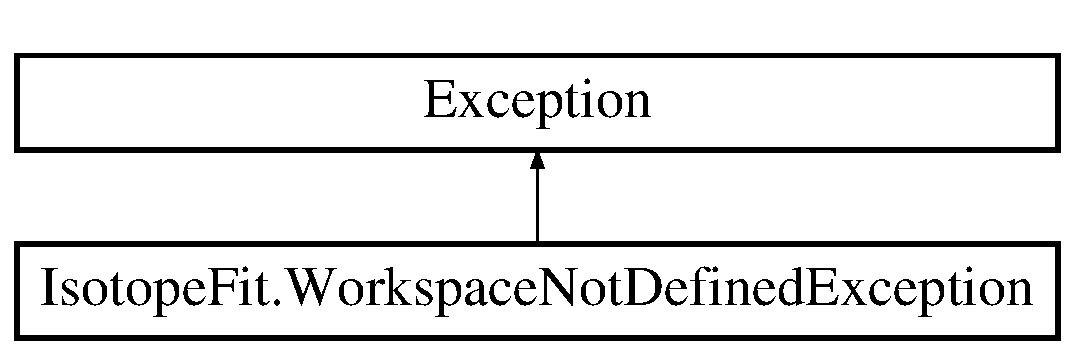
\includegraphics[height=2.000000cm]{class_isotope_fit_1_1_workspace_not_defined_exception}
\end{center}
\end{figure}
\subsection*{Public Member Functions}
\begin{DoxyCompactItemize}
\item 
\mbox{\Hypertarget{class_isotope_fit_1_1_workspace_not_defined_exception_a3b995d53506b67b380bc2c54754321dc}\label{class_isotope_fit_1_1_workspace_not_defined_exception_a3b995d53506b67b380bc2c54754321dc}} 
{\bfseries Workspace\+Not\+Defined\+Exception} (string message)
\item 
\mbox{\Hypertarget{class_isotope_fit_1_1_workspace_not_defined_exception_a53f2fd5a9c57a46f898b632963a2c406}\label{class_isotope_fit_1_1_workspace_not_defined_exception_a53f2fd5a9c57a46f898b632963a2c406}} 
{\bfseries Workspace\+Not\+Defined\+Exception} (string message, Exception inner)
\end{DoxyCompactItemize}
\subsection*{Protected Member Functions}
\begin{DoxyCompactItemize}
\item 
\mbox{\Hypertarget{class_isotope_fit_1_1_workspace_not_defined_exception_aff29f81b2cf445dd91deb0f2e58c83e3}\label{class_isotope_fit_1_1_workspace_not_defined_exception_aff29f81b2cf445dd91deb0f2e58c83e3}} 
{\bfseries Workspace\+Not\+Defined\+Exception} (System.\+Runtime.\+Serialization.\+Serialization\+Info info, System.\+Runtime.\+Serialization.\+Streaming\+Context context)
\end{DoxyCompactItemize}


\subsection{Detailed Description}


Definition at line 11 of file Workspace\+Exceptions.\+cs.



The documentation for this class was generated from the following file\+:\begin{DoxyCompactItemize}
\item 
Isotope\+Fit\+Lib/\+Workspace/Workspace\+Exceptions.\+cs\end{DoxyCompactItemize}

\hypertarget{class_isotope_fit_1_1_workspace_1_1_workspace_status}{}\section{Isotope\+Fit.\+Workspace.\+Workspace\+Status Class Reference}
\label{class_isotope_fit_1_1_workspace_1_1_workspace_status}\index{Isotope\+Fit.\+Workspace.\+Workspace\+Status@{Isotope\+Fit.\+Workspace.\+Workspace\+Status}}


Class for storing the \hyperlink{class_isotope_fit_1_1_workspace}{Workspace} status flags and message log for the user.  


\subsection*{Properties}
\begin{DoxyCompactItemize}
\item 
\mbox{\Hypertarget{class_isotope_fit_1_1_workspace_1_1_workspace_status_a65fb659d552aa2c15400d40e09396229}\label{class_isotope_fit_1_1_workspace_1_1_workspace_status_a65fb659d552aa2c15400d40e09396229}} 
bool {\bfseries Baseline\+Corrected}\hspace{0.3cm}{\ttfamily  \mbox{[}get, set\mbox{]}}
\item 
\mbox{\Hypertarget{class_isotope_fit_1_1_workspace_1_1_workspace_status_a2f66d7e59cd164d2275e33ec3569eb5a}\label{class_isotope_fit_1_1_workspace_1_1_workspace_status_a2f66d7e59cd164d2275e33ec3569eb5a}} 
bool {\bfseries Mass\+Offset\+Corrected}\hspace{0.3cm}{\ttfamily  \mbox{[}get, set\mbox{]}}
\item 
\mbox{\Hypertarget{class_isotope_fit_1_1_workspace_1_1_workspace_status_afa27a586f87d2d550fe9f45f0775a0f7}\label{class_isotope_fit_1_1_workspace_1_1_workspace_status_afa27a586f87d2d550fe9f45f0775a0f7}} 
bool {\bfseries Design\+Matrix\+Built}\hspace{0.3cm}{\ttfamily  \mbox{[}get, set\mbox{]}}
\item 
\mbox{\Hypertarget{class_isotope_fit_1_1_workspace_1_1_workspace_status_a15a3a16c34a8f8df6cdb7bcbc9118e53}\label{class_isotope_fit_1_1_workspace_1_1_workspace_status_a15a3a16c34a8f8df6cdb7bcbc9118e53}} 
bool {\bfseries Abundances\+Fitted}\hspace{0.3cm}{\ttfamily  \mbox{[}get, set\mbox{]}}
\item 
\mbox{\Hypertarget{class_isotope_fit_1_1_workspace_1_1_workspace_status_aa1e34a4e9627d00e654a47aa13d44629}\label{class_isotope_fit_1_1_workspace_1_1_workspace_status_aa1e34a4e9627d00e654a47aa13d44629}} 
List$<$ double $>$ {\bfseries Message\+Log}\hspace{0.3cm}{\ttfamily  \mbox{[}get, set\mbox{]}}
\end{DoxyCompactItemize}


\subsection{Detailed Description}
Class for storing the \hyperlink{class_isotope_fit_1_1_workspace}{Workspace} status flags and message log for the user. 



Definition at line 530 of file Workspace.\+cs.



The documentation for this class was generated from the following file\+:\begin{DoxyCompactItemize}
\item 
Isotope\+Fit\+Lib/\+Workspace/Workspace.\+cs\end{DoxyCompactItemize}

%--- End generated contents ---

% Index
\backmatter
\newpage
\phantomsection
\clearemptydoublepage
\addcontentsline{toc}{chapter}{Index}
\printindex

\end{document}
